%%%%%%%%%%%%%%%
% START COPY %%
%%%%%%%%%%%%%%%

%\epigraph{\selectlanguage{german} \glqq Die Existenz von Mischformen bedeutert jedoch nicht, daß die Trennung von »Zeichen« und »Zeichnung« verwischt werden soll. Im Gegenteil: Daß innerhalb der Mischformen der Zeichenanteil und der graphische Aspekt sich trennen lasses, zeigt gerade, daß es sich um zwei grundverschiedene Kategorien handelt.\grqq \selectlanguage{english}}{György Ligeti, 1965}


\epigraph{\singlespacing ``The existence of mixed forms does not, however, mean we ought to blur the division between `sign' and `illustration.' On the contrary, the fact that the sign component can be separated from the graphic aspect [...] is itself a demonstration that we are dealing with two fundamentally different categories.''}{György Ligeti, 1965, tr. Edmund Griffiths.}


%    \small
%    \begin{itemize}
%        \item \texttt{\textbf{\textcolor{red}{red = construction notes}}}
%        \item \texttt{\textbf{\textcolor{blue}{blue = I want this somewhere but maybe not here?}}}
%        \item \texttt{\textbf{\textcolor{ForestGreen}{ForestGreen = an idea that, to the best of my ken, is mine}}}
%    \end{itemize}
%    \normalsize

%\section{Introduction}

    In the previous chapter, I used a rapid historical gloss to illustrate an important narrative arc in Western art music's technological development. Specifically, I aimed to chart the ebb and flow of notation's relative sonic determinacy---the openness and fixity of our shared musico-graphic signs. While much of this effort was dedicated to tracking changes in the common practice notation serving as most literate musicians' lingua franca, the final section of the chapter addressed a few of the varieties of new notation which seemed to spring up \textit{ex nihilo} in the 1950s and 1960s. To my mind, the most interesting and under-analyzed of these and subsequent new notations feature robust encoding schemes which provide specific shape and color to a musical work---while at the same time permitting a great deal of creative latitude on the part of the work's interpreter(s).
    
    This chapter is ultimately intended to address the analytic issues posed by the arrival of these bespoke ``open'' notations and to move toward new ways of thinking about their form and function which avoid the murky, obscurant language often featuring in their discussion. To wit, the specific goal I have set for this chapter is the development of a working typology of notations; one able to fold in the variety of traditional methods of music encoding, but one specifically aimed at disambiguating the variety of extant open notations so prevalent in the composition of the twentieth and twenty-first centuries. Only so armed may we then begin to make sense of the more complex open works which spurred on this research---works which may operate on many simultaneous levels of fixity, employing several different encoding schemes over the course of a single piece, a single section or a single measure.

    To that end, I'll begin by discussing what I take to be the most pressing issues facing our clear-eyed assessment of music notation, moving from most general to most specific. Specifically, I'll first address our ``common-sense'' notion of notational semantic content; putting forward a new way of thinking about notation-as-symbol so as to find a shared vocabulary with which to discuss both traditional and neo-notation on the same terms. Next, I'll interrogate concepts of openness in music composition; specifically highlighting common takes on the ``open work,'' generally, and on ``graphic notation,'' which I take to needlessly complicate our understanding of this notation's function. Following this, I will highlight those few scholarly efforts which seem to take positive steps toward our goal---with special emphasis on a critically under-cited essay which I think does a great deal of the work in describing our desired typology. Ultimately it is this source which I'll use to catalyze the development of a refined model.


\section{Base-level function of music notation}

    \begin{smallquote}
        In music notation, sounds are represented by small circles (or ovals) called notes. Notes can be high or low, and they can be short or long. The higness [sic] or lowness of the note is its pitch. To represent high and low pitches, notes are placed high or low on the staff, the five horizontal lines going across the page.\autocite{Wood_2015}
    \begin{center}
    \noindent\rule{1cm}{0.4pt}
    \end{center}   
        Notation is a recognised system of symbols (essentially marks on paper) that visually represent a music or sound idea. Standard notations are well-known, clearly defined structures that are able to communicate sound information in a functional and precise manner.\autocite{debbielyddon_2015}
    \begin{center}
    \noindent\rule{1cm}{0.4pt}
    \end{center}
        Printing music on a page allows a composer to convey information to a musician who will ultimately perform that composer’s work. The more detailed the musical notation, the more precise a performer will be. In this sense, musical notation is no different from printed text.\autocite{Music_101}
    \begin{center}
    \noindent\rule{1cm}{0.4pt}
    \end{center}
        \end{smallquote}
        
    As promised, I would like to begin by revisiting a few of our initial assumptions given at the beginning of the last chapter, specifically as regards the foundations of the function of music notation and of its potential to mediate musical performances. The ability to meaningfully consider complex new works which often combine several distinct varieties of notation in a single score is entirely contingent on an understanding of what, at a basic level, these notations are doing---i.e. what they encode and transmit.
    
    I provide the above inscriptions as an interesting  sampling of the variety of extant definitions of ``music notation.'' The above public-facing, decidedly non-academic definitions were specifically chosen for the way they seem to get at the ambient, unexamined sense of what it is we use notation \textit{for}. It is particularly interesting to note their discrepancies: The first takes notation to directly refer to sounds---though it is unclear whether these are meant to be virtual or real---and makes sure to include the mapping between spatial dimensions on the page and height in frequency space. The second mentions ``music-'' and ``sound-ideas'' as potential referents for notation, though does not go into detail as to their differences. Here, notations are structures for the communication of this sound data from composer to performer such that the performer, having formed a clear mental image of what sound the composer is seeking, will be able to bring it into being. The third, on the other hand, does not refer to sound at all. Like the second, it emphasizes that notation is a means of information conveyance between a communicator and communicatee. However, precisely what \textit{sort} of information notation actually bears is left unspecified. Interestingly, it also immediately appeals to our notion of precision---implying that there exists some ideal virtual music toward which notation aims; carrying with it the implicit goal that performers should get as close to it as possible. These represent three distinct ways of thinking about our everyday interactions with music notation---none of which, alone, allow us to describing using uniform vocabulary the manifold forms of notation we observed in the last chapter.
    
    David Gutkin, in a paper I'll return to later in this chapter, hints at a sort of solution:

        \begin{smallquote}
            But might not any musical notation and not solely particular avant-garde scores or tablature be understood as the prescription of action rather than, or at least as well as the coding of sound? Even if notation does not always mimetically or analogically depict physical movements \textit{per se}, culturally significant graphic marks are only ever operative as imperatives to act.\autocite{Gutkin}
        \end{smallquote}

    In the following section, I will argue for just such a model of notation-interaction---one which de-centers common notions of sound-signification in favor of mediation of fields of potential musical action. The aim of this model is not to replace common parlance or overturn centuries of received wisdom pertaining musical inscription at large, but rather to enable a more precise discourse---especially as regards complex, multiform neo-notation that characterizes so many fascinating works today. 
    
    \subsection{Notation as imperative to act}
    
    To begin with, I will refer back to Mieko Kanno's definition with which we began the previous chapter. Per Kanno, music notation serves generally to ``describ[e] musical works and giv[e] specific instructions for them to be realized.'' Earlier, I refined (genericized) this definition slightly by allowing that music notations merely be coherently ``oriented toward an existing [...] or virtual [...] musical product'' given that there exist many music notations which were never intended to allow for realization of a work (Rainer Wehinger's famous \textit{ex post facto} ``graphic'' score for György Ligeti's \textit{Artikulation}, for instance). While these definitions served as a good launchpad for our discussion, neither of them give any idea as to the mechanism by which notation ``describes'' or is ``oriented'' toward sonic products. Though the article itself is fairly comprehensive, the head-line definition in the \textit{Grove} entry for ``Notation'' is similarly vague. For its primary author, Ian Bent, notation taken whole is simply some ``visual analogue of musical sound, either as a record of sound heard or imagined, or as a set of visual instructions for performers.''\autocite{Bent_2014} Elegant, broad-level definitions like these necessarily fail to get us any closer to an understanding of the objects to which elements of music notation actually refer. For that, we must turn to discussions of notational semiotics. Luckily, a good starting point is not far away. In a later section of the article, Bent elaborates:

        \begin{smallquote}
            A musical notation requires, in essence, two things: an assemblage of ‘signs’ and a convention as to how those signs relate to one another. A written musical notation requires further a spatial arrangement of the signs on the writing surface that makes a ‘system’ of the assemblage; it is this system that forms an analogue with the system of musical sound, thus enabling the signs to ‘signify’ individual elements of it.\autocite[Section II.1]{Bent_2014}
        \end{smallquote}

    This strikes closer to the heart of the question. Here Bent establishes the position that music notation (taken whole) serves as a ``visual analogue'' of actually-existing music. A system of notation comprises signs (what I've been generically calling ``glyphs'') and a syntax through which those signs are perceived and understood. Implicit in Bent's argument, though, is the assumption that the sound-system's referents (signified by the assemblages which form our notations) are \textit{themselves} sounds. 
    
    To clarify: Per the paradigmatic ``standard'' model of composition: A composer conceives of music in some way and represents it in a score, then hands it off to a performer who creates music using the score as a sort of ``recipe,'' hopefully satisfying everyone in the process. Semantically speaking, though, the score serves as a sort of black box of representation---while it's clearly desirable that a score (as an individual entity) should bear some representative orientation toward some body of sound, either past, future, or potential, it is not altogether trivial precisely what the composer is encoding and sending and precisely what the performer is receiving when this process of representation takes place. Given the definitions we've seen, one might naïvely imagine that (i) a composer simply conceives of ``pure sound,'' in some arrangement, (ii) determines which symbols from his repertory would be best to represent that sound and commits them to paper, after which (iii) a performer interprets these symbols---similarly taking them as signifying particular sounds which they must dutifully bring into existence. The performer then realizes these sounds of the type and ordering the composer intended and everyone is happy. This model, however, has some critical flaws which expose the inadequacy of the notion that music notation somehow represents sound in the way that a noun represents a person, place, or thing.\footnote{
        Let us be clear that sounds (as they actually exist) are physically- and temporally-extended \textit{things}---highly complex and specific in form. I take it that even the strictest ``sound-semanticist'' would not argue that the familiar glyphs on the page are meant to refer to some \textit{specific} sound (e.g. of the form \{A442 at 80dB begun March 9th 1972 at 14:30:26 and ending March 9th 1972 at 14:30:27.5\}. Rather, I take it that they would argue that the symbol on the page directly refers to some internally-audiated sound which bears a reasonable resemblance to some sound \textit{also} familiar to the performer.
        }
    
    First, it is often the case that a composer does not intend a particular sound at all, but what we might generically call a ``process''---for instance some harmonic function. If I write B$^{\flat-7}$ on the lead sheet I'm composing, it's not because I'm imagining some particular sound, but because I desire harmonic functionality of a particular form from my rhythm section or soloist. Fulfilling that harmonic role faithfully could yield any number of resultant sounds---any of which would satisfy the composer. Similarly, a composer might intend not a sound, but a particular sort of physical gesture \textit{irrespective} of what sound results. Figure~\ref{fig:pression} illustrates an excerpt culled from Helmut Lachenmann's brilliant \textit{Pression} for unaccompanied 'cello, which, per Paul Griffiths ``is typical of Lachenmann's work of this period in its concentration on irregular techniques, and thereby on the physical mechanism by which the sounds are produced.'' Below, we see his novel proportional notation which specifies the non-sounding movement of the left hand separately from the sounding movement of the bow. Given that an audience member three rows back from the performer may not even be able to hear the thin, breathy sound emitted, it is not too far flung to imagine that Lachenmann penned this gesture for the theatricality of its movement rather than for the precise attributes of its sonic byproducts. Here, neither the intent nor that which is transmitted by the notation is sound proper.\autocite{Griffiths_2011}

        \begin{figure} 
            \centering
            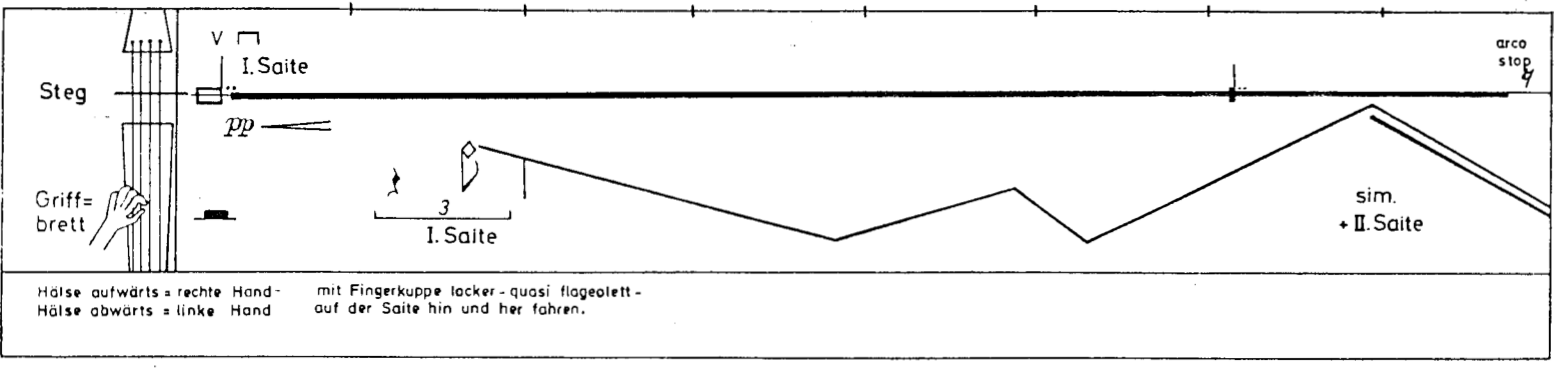
\includegraphics[width=.99\textwidth]{images/chapter2/pression1.png}
            \captionsetup{width=.5\textwidth}
            \caption[First system of Helmut Lachenmann's \textit{Pression} (1969) demonstrating non-sounding ``gestural'' notation (lower jagged line) which modifies sounding notation (upper solid line).]{First system of Helmut Lachenmann's \textit{Pression} (1969) demonstrating non-sounding gestural notation (lower jagged line) which modifies sounding notation (upper solid line).\footnotemark}
            \label{fig:pression}
        \end{figure}
            \footnotetext{\fullcite[]{Lachenmann_1969}}

    Indeed, especially in contemporary music there are many such symbols which clearly yield sound via their interpretation but for which we would struggle to clearly identify a sonic referent. What ``sound'' is indicated by a figured-bass symbol? Likewise, what ``sound'' is indicated by the boxes in Feldman's \textit{Projections} series? The rectangles in \textit{December 1952}? Further, if notation is to refer specifically to concrete sounds it becomes non-trivial to define the inner workings of ``more fixed'' or ``more open'' notations---categories which clearly function  in practice. Sound (at least under our common usage of the term), whether imagined or issued, cannot be any more or less fixed than it is. A sound is merely an end product of the process notation inscribes. Simply put, our common-sense understanding of notation's ``fixity'' or ``openness'' can not obtain if we take notations to formally refer to sounds proper. In this light, I would like to tentatively put forward an alternative model of notational semantics in order to facilitate discussion of the open works at the core of this project. The following is a semi-formal elaboration of my argument:

    % \begin{notestuff}
    %     (unsure of the best way to format this... I want to illustrate the logical flow, but maybe bullets/numerals are too strange...)
    % \end{notestuff}

    \begin{center}
    \noindent\rule{3cm}{0.4pt}
    \end{center}   

        \begin{itemize}[leftmargin=*, label=--]
        
        \item Music notation is typically used to generate or archive music. It seems correct that music notation, properly arranged, should by and large \textit{represent} in some way its resultant musical products (i.e. virtual or actually-existing sounds). A score---some meaningful, cohesive arrangement of notation---serves as a ``recipe'' allowing for the creation or recreation of an imagined complex of sounds extended in time. We might think of the score, its encoding procedure, and its resultant (or potentially resultant) sounds as together forming a conceptual whole. An important misconception which might arise from this ${score} \rightarrow {music}$ mapping, though, is that individual glyphs \textit{congruently} map to individual sounds---i.e. that there exist one-to-one mappings between units of notation and the expected sounds which ought to result from their reading.
            
        \item During the encoding process, symbols are chosen by a composer (from a repertory of such symbols) on the basis of their results---i.e. the sounds, gestures, or procedures which would result from their interpretation. However, we should be very cautious about making the claim that the symbols are chosen because they necessarily \textit{refer directly} to some desired sounds.
            
        \item The score's downstream sonic products, after all, only result in practice via some interaction (be it a tight or a loose reading) between a performer and the notation provided by the composer. The performer's body and instrument stand between score and sound---thus the glyph \{$\vcenter{\hbox{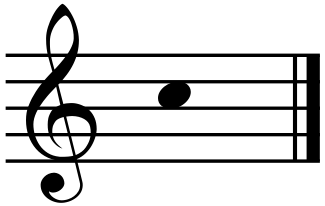
\includegraphics[width=1.2cm]{images/chapter2/c5raw.png}}}$\} in practice does not ``neutrally'' stand in for some platonic, un-sounded C5, but rather results in a C5 as brought into existence by some sounding body. As a convenient shorthand, we think of it as referring to raw pitch data, but insofar as we are discussing notation oriented toward \textit{performance}, this is not the case.
            
        \item For instance, it should be unambiguous that the individual note-glyph \{$\vcenter{\hbox{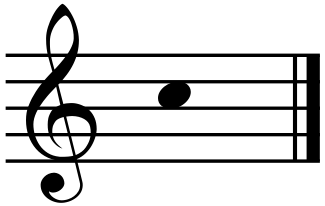
\includegraphics[width=1.2cm]{images/chapter2/c5raw.png}}}$\} does \textit{not} refer to a sound. Given the traditional understanding of how music notation syntax works, there's not enough information to reproduce a particular imagined sound from the information given. However, in many literate music traditions, perfectly valid scores might be constructed entirely of such ``bare'' notes, as is the case with many of the works in Anthony Braxton's ``Ghost Trance Music'' series (see Figure~\ref{fig:ghosttrance1}).
    
        \begin{figure} 
            \centering
            \fbox{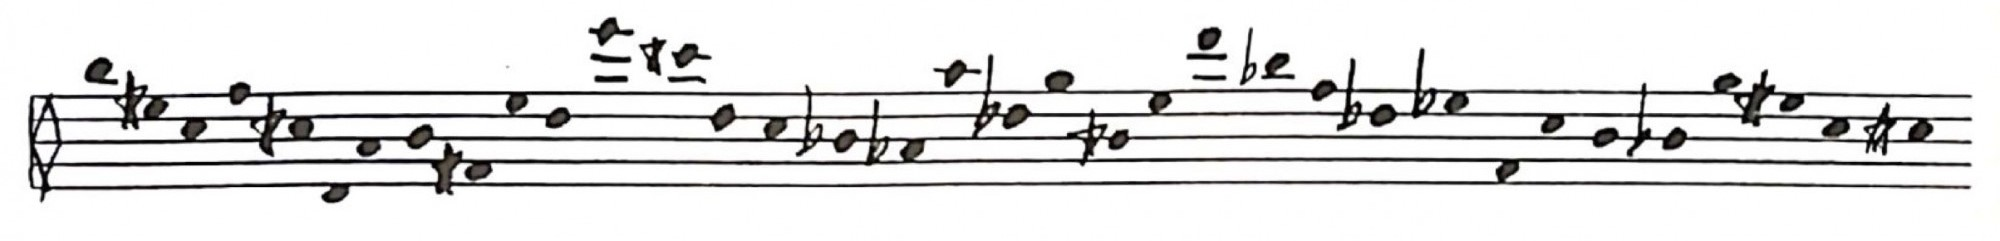
\includegraphics[width=.9\textwidth]{images/chapter2/ghosttrance2.jpg}}
            \captionsetup{width=.5\textwidth}
            \caption[Excerpted system from Anthony Braxton's \textit{Composition No. 193} which features long stretches of unadorned noteheads and bespoke ``diamond'' clefs and ``star'' accidentals.]{Excerpted system from Anthony Braxton's \textit{Composition No. 193} which features long stretches of unadorned noteheads and bespoke ``diamond'' clefs and ``star'' accidentals.\footnotemark}
            \label{fig:ghosttrance1}
        \end{figure}
            \footnotetext{Reproduced courtesy of \fullcite[]{Cauwenberghe_2021}. Due to the complex nature of Braxton's graphic titles, I will be abbreviating them as necessary with his self-imposed catalog numbers.}
    
        \item One might assert instead that notation refers to specific sounds only when enough clear information is provided (per the rules of our system as we understand it) to fulfill the ``recipe'' with a particular instrument and with a particular tempo and dynamic. After all, I can much more clearly imagine the sound which would result from \{$\vcenter{\hbox{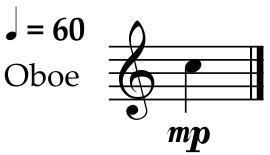
\includegraphics[width=2cm]{images/chapter2/c5oboe.png}}}$\} than from its unadorned cousin.
            
        \item Unfortunately, this is still an insufficient model. Humans cannot realize symbols identically each time; even with this greater degree of specificity, there will always be discrepancies (even large discrepancies) between repeated realizations. Each symbol or complex of symbols either explicitly or implicitly carries with it a degree of latitude as to what constitutes a valid or acceptable realization. \{$\vcenter{\hbox{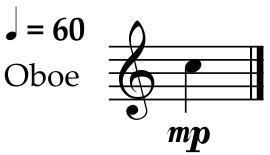
\includegraphics[width=2cm]{images/chapter2/c5oboe.png}}}$\} might be cut off 20 milliseconds short of the mathematically called-for duration, it might be flat or sharp by 10 cents, it might be slightly louder or softer, it might be performed with light or no vibrato, etc.
            
        \item It is therefore impossible to point to any particular sound which serves as the referent for any complex of music-notation symbols. As such, I would like to propose an alternative model; specifically, one in which notation's referent is instead conceived as a virtual set of sound-producing actions which could plausibly result from the notation's rendering in performance. In the previous example, the glyph-complex \{$\vcenter{\hbox{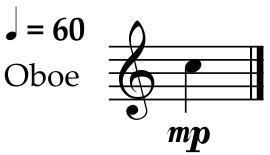
\includegraphics[width=2cm]{images/chapter2/c5oboe.png}}}$\} would refer to a set which includes all of the given potential realizations as well as any others which would be considered faithful. I'll use the term ``field of potential'' (FOP) to refer to this set of appropriate realizations which serves as the referent to a notational glyph.
            
        \item As such, we no longer need to adorn a bare \{$\vcenter{\hbox{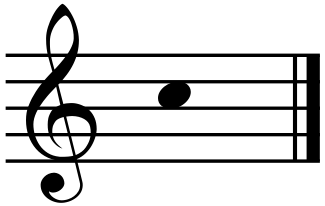
\includegraphics[width=1.2cm]{images/chapter2/c5raw.png}}}$\} (which would and has served as a structurally-complete notation all by itself) with all of these other symbolic trappings (dynamic, tempo, etc.) in order to meaningfully describe a referent for a particular glyph. The bare C5's referent, in other words \textit{contains} the referent of \{$\vcenter{\hbox{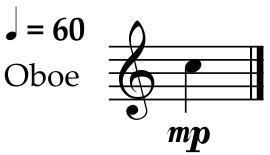
\includegraphics[width=2cm]{images/chapter2/c5oboe.png}}}$\} as well as any other potential realization of \{$\vcenter{\hbox{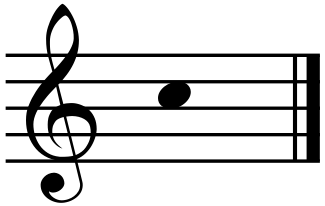
\includegraphics[width=1.2cm]{images/chapter2/c5raw.png}}}$\}.
        
        \end{itemize}

    \begin{center}
    \noindent\rule{3cm}{0.4pt}
    \end{center}   

    Of course, this argument itself raises some important questions. What, first of all, defines the scope and content of this field of potential action? If we are to suspend our notion that somehow notational glyphs map one-to-one with intended sounds, we must at the same time adopt a new model of how notation-mediated communication \textit{works}. As with any semantic content, notation's field of potential is multiply determined via a complex of (i) the ``encoder's'' intent, (ii) the code regulating the sign's usage, and (iii) the recipient's reading of the sign. On the part of the composer, the FOP is defined by some intentional \textit{sound- or process-concept} (S/PC) which he encodes to the best of his ability using the glyphs at his disposal. Under this model, the process (for a typical sound-concept) proceeds as follows:

        \begin{smallquote}
            \begin{itemize}[label=--]
                \item A composer internally audiates a sound for oboe, based on his past experience of ``oboeness,'' (i.e. develops a sound-concept) and decides to encode it for a performer to reproduce.
                \item He must then ask himself two things:
                    \begin{enumerate}
                        \item Does the chosen glyph's implied FOP include the sound he has audiated?
                        \item How much discrepancy between his audiated sound and the actual performed sound would be permissible?
                    \end{enumerate}
                \item If the chosen glyph's FOP contains the imagined sound \textit{and} allows only for permissible discrepancy given the established code agreed upon by composer/performer, then the glyph suffices.
                \item If, on the other hand, the glyph's FOP contains the imagined sound, but the potential discrepancy between audiated sound and performed sound is too great, the composer must further \textit{restrict} the FOP in some way---either with additional symbolic modifiers (\textbf{\textit{mp}}, $\quarterNote$=60, etc.) or with verbal/textual instructions.
            \end{itemize}
        \end{smallquote}

    Crucially, this procedure holds true independent of the degree of fixity inherent in the system of notation. If music notation were to somehow point to sound directly, we would have to posit entirely different modes of signification between ``closed scores'' which refer directly to fixed, predictable virtual sound and ``open scores'' which grant the performer some degree of latitude in realization. That certain notations, be they systems or individual glyphs, permit more leniency in interpretation (i.e. are more open) should be uncontroversial. This being the case, though, we would need a way of describing the represented sound as \textit{itself} being more or less definite depending on whether its associated sign were open or closed---ultimately an unenviable position when compared with the simpler alternative. Below I have prepared two time-oriented ``flow'' diagrams illustrating the standard composer/performer interaction---one under the ``naïve'' model (Fig.~\ref{fig:naïvediagram}) and one under my amended model (Fig.~\ref{fig:amendeddiagram}). Translations of the relevant relationships follow the figures.\footnote{
        A couple of caveats for these interaction charts: First, this is meant to be a model illustrating the simplest possible composer/notation/performer interaction---it does not purport to represent \textit{all} such interactions. In practice, obviously, there are complex feedback mechanisms (e.g. player feedback in rehearsal, inter-musician communication, etc.) which would change the whole interaction structure. 
        
        Second, this is meant to be an interaction between a composer and a \textit{single} performer. The model could just as well be expanded to include an arbitrary number of agents but for the purposes of illustration I thought it best to keep things as simple as possible. 
        
        Third, I marked $S^*_P$ optional for the fact that, it seems, we could conceive of a scenario where the performer ``mechanically'' reproduces notation which they are capable of executing but which is too complex to audiate inwardly. Alternately, the composer may have encoded a process-concept which is likewise reproducible by the performer but which is so opaque it fails to reveal itself conceptually. In either case, a ``reflected'' sound/process-concept is not strictly necessary for the model; hence the broken line.
        
        } 

%        \begin{notestuff}
%            I need a small paragraph here or at least a generous footnote describing the role of ``syntax'' in the amended model I put forward below. It just comes out of nowhere and does a lot of work. Also, I drew an ``influence arrow'' from ``syntax'' only to the gamma-complex. But shouldn't it kind of point everywhere??
%        \end{notestuff}

        \begin{figure} 
            \centering
            \fbox{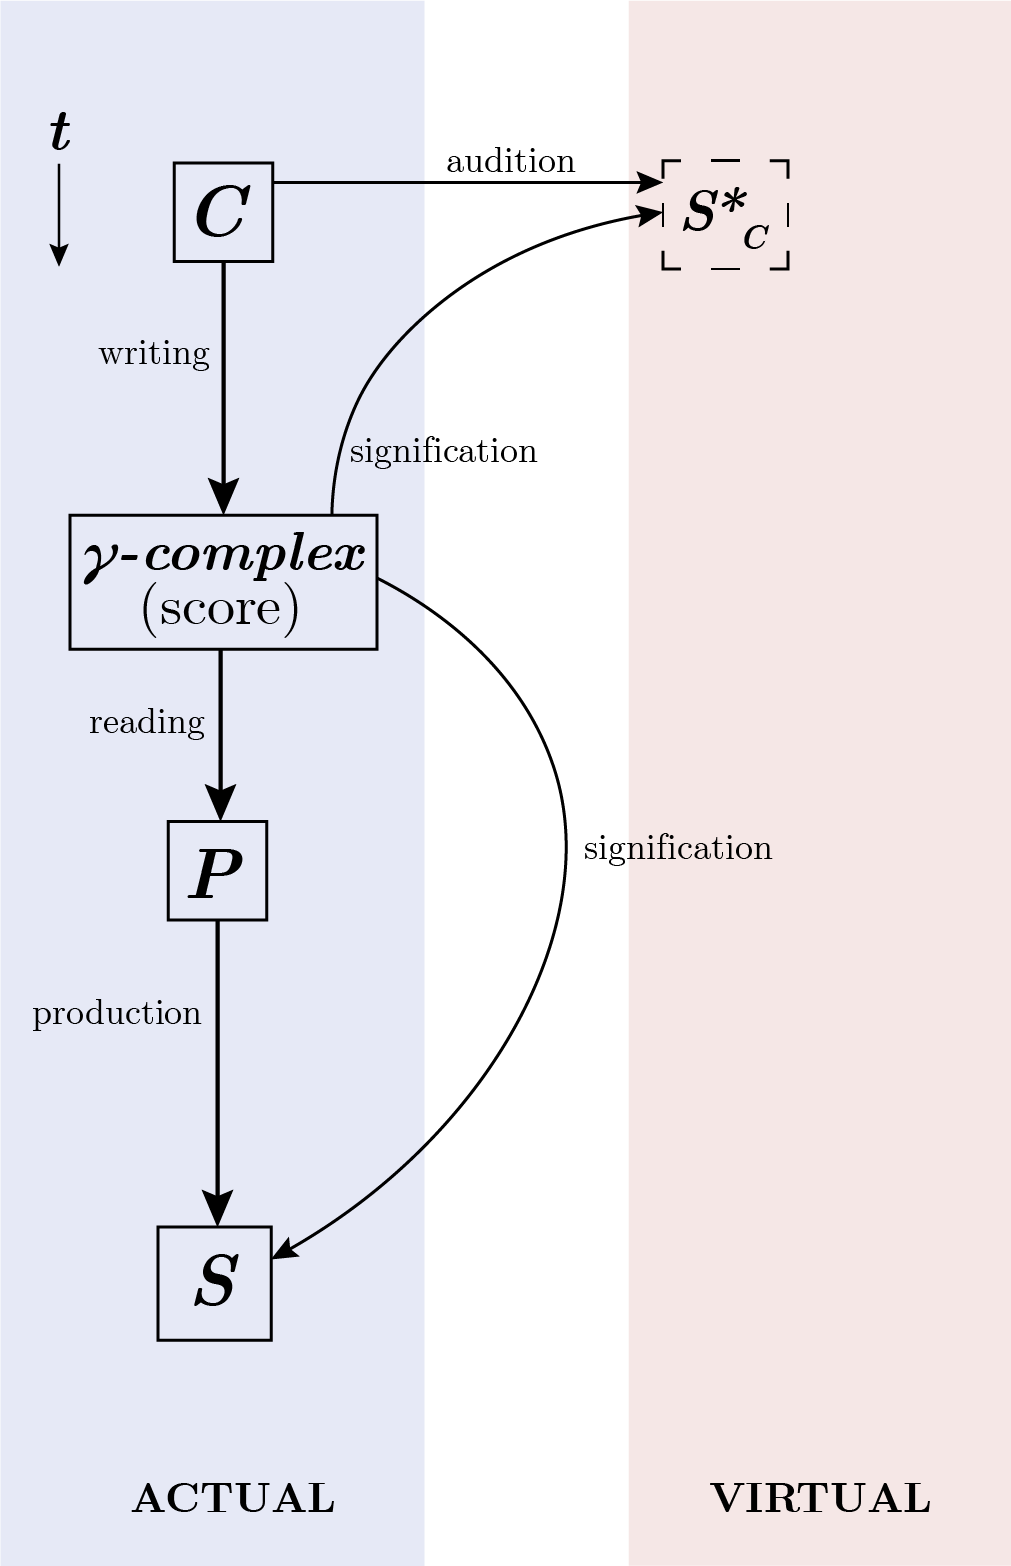
\includegraphics[width=.5\textwidth]{images/chapter2/2-3x.png}}
                
                \begin{smallquote}
                    \begin{center}
                        \textit{``Naïve'' Process}
                    \end{center}
                
                    \begin{enumerate}
                        \item A composer ($C$) \textbf{audiates} a sound-concept ($S^*_C$) which s/he wishes to realize in sound.
                        \item S/he \textbf{writes} the score---a complex of glyphs ($\gamma$) intended to yield the imagined $S^*_C$ at some future time.
                        \item A player ($P$) \textbf{reads} the score, forming a mental image which matches that devised by the composer ($S^*_C$).
                        \item $P$ then \textbf{produces} corresponding sound $S$.
                        \item To the outside observer, $\gamma-complex$ \textbf{represents} the final sound $S$ produced as well as the sound concept $S^*_C$ originally devised.
                    \end{enumerate}
                \end{smallquote}

            \captionsetup{width=.5\textwidth}
            \caption{``Naïve'' notation interaction model.}
            \label{fig:naïvediagram}
        \end{figure}

            
        \begin{figure} 
            \centering
            \fbox{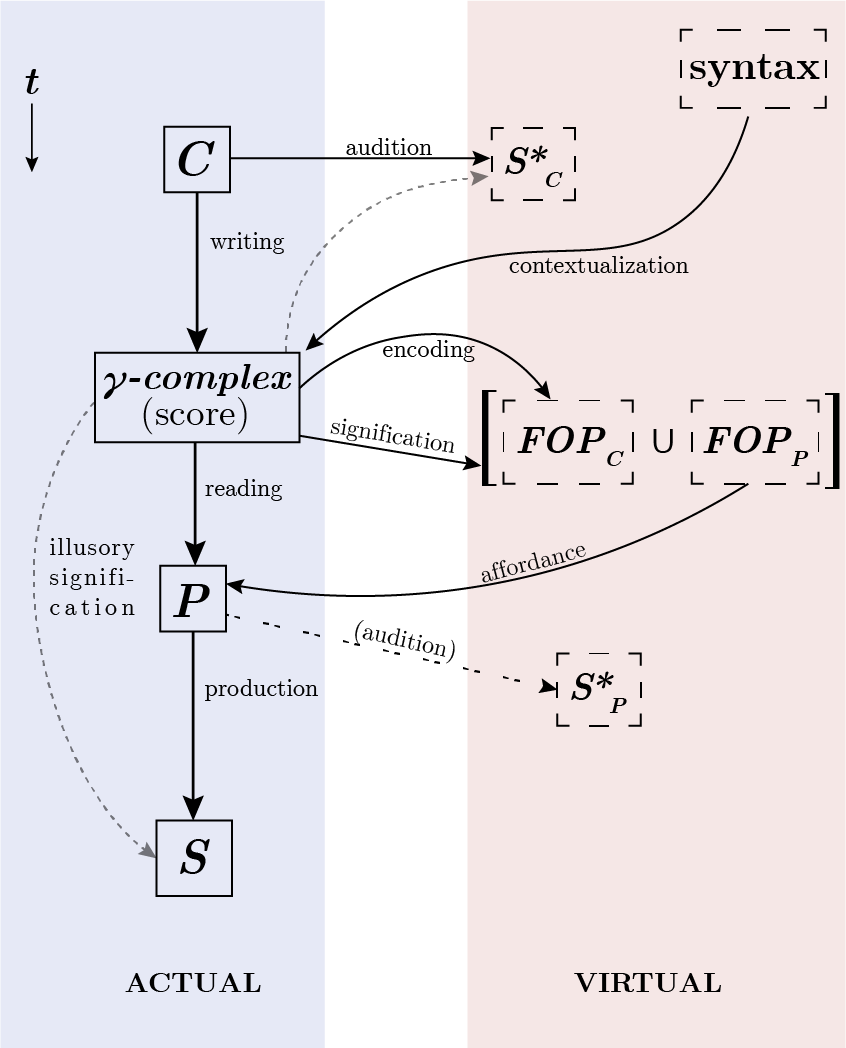
\includegraphics[width=.65\textwidth]{images/chapter2/signification_diagram_fix.png}}
                
                \begin{smallquote}
                
                    \begin{center}
                        \textit{Amended Process}
                    \end{center}
            
                    \begin{enumerate}
                        \item Syntax \textbf{organizes} the whole interaction and is familiar to both composer ($C$) and performer ($P$), whether it is part of the received structure of music notation or newly communicated in the score.\footnotemark                            
                        \item $C$ \textbf{audiates/devises} some sound/process-concept ($S^*_C$) which he would like to hear $P$ perform.
                        \item $C$ \textbf{writes} the score---a complex of glyphs ($\gamma$-complex)---such that  their realization might bring about an instance of $S^*_C$. (That is, such that a field of potential $FOP_C(\gamma)\Rightarrow S^*_C$ where ``$\Rightarrow$'' is a relation meaning ``fulfills'').
                        \item $P$ \textbf{reads} $\gamma-complex$, which affords him/her $FOP_P$.
                            \begin{enumerate}
                                \item To an outside observer, $C$'s $\gamma-complex$ can then be said to represent the union of $FOP_C$ and $FOP_P$.
                                \item $P$ may him/herself \textbf{audiate/devise} $S^*_P$ such that $S^*_P \approx S^*_C$, though it's not strictly necessary.
                            \end{enumerate}
                        \item $P$ executes $\gamma-complex$, selecting a gesture $g$ (such that $g \in FOP_P$), which \textbf{produces} sound.
                    \end{enumerate}
                \end{smallquote}

            \captionsetup{width=.5\textwidth}
            \caption{Amended notation interaction model.}
            \label{fig:amendeddiagram}
        \end{figure}
            \footnotetext{ 
                        One final qualification: Where elsewhere I have attempted to be as precise as possible when choosing the language with which to describe these notation-interaction models, here I have somewhat callously included the catchall module labelled ``syntax'' as a way of hand-waving the many \textit{a priori} factors which influence the way notation is used to encode/decode music. To be more specific, I take this ``syntax'' to be a global variable comprising, for instance, (a) the extent to which the composer and performer were formally trained in the use of the notation scheme, (b) their musical upbringing (Am I to play these triplets the French or Italian way?), (c) personal taste (How furious is \textit{furioso}?), (d) the notation's graphic trace (How well is the piece engraved? Are the symbols legible?), as well as many other factors. Naturally there will always be some discrepancy (ranging from inconsequential to game-changing) between the composer's received syntax and the performer's based on their entirely distinct lived experiences.
                                    
                        In addition, I have drawn an arrow from ``syntax'' to the $\gamma$ complex in order to depict (very generally) the way these syntactic elements influence the artifact that is the score, though perhaps it would be more correct to point this directional influence at the ``audition,'' ``writing,'' and ``reading'' processes themselves.
                        }

    Per my earlier comment, it should go without saying that this amended view of notation-signification is not meant to supercede the common-sense way we talk about or interact with notation in the course of our everyday musical experiences. Instead, couching the content and function of notation in terms of fields of potential action should allow us to assess complex, multi-notational works (for instance, Anthony Braxton's \textit{Composition No. 76} excerpted in Fig.~\ref{fig:Braxtonex}) with greater clarity; a task I'll be attempting in Chapter 3.

        \begin{figure} 
            \centering
            \fbox{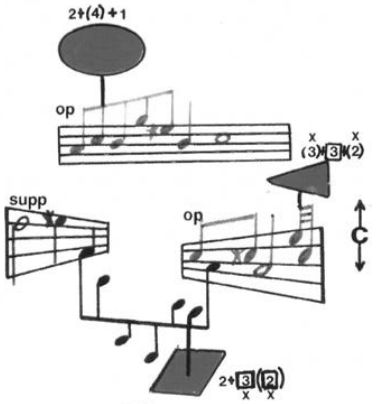
\includegraphics[width=.5\textwidth]{images/chapter2/76no1.png}}
            \captionsetup{width=.5\textwidth}
            \caption[Excerpt of module ``E3'' from Anthony Braxton's \textit{Composition No. 76} (1978) demonstrating multiple concurrent forms of notation operating at several degrees of openness.]{Excerpt of module ``E3'' from Anthony Braxton's \textit{Composition No. 76} (1978) demonstrating multiple concurrent forms of notation operating at several degrees of openness and semanticity.\footnotemark}
            \label{fig:Braxtonex}
        \end{figure}
            \footnotetext{\autocite{Braxton_Comp_76}}

    In advance of this, though, it is crucial that we first consider our received notion of what, precisely, constitutes an ``open work.'' Given that our stated goal is the development of a working typology, it is worth assessing those sources which posit new forms of notation; in practice, usually ones designed for the construction of new, sonically indeterminate works. Writers with insight into these new forms of composition often have views on their attendant notations which are worth examining in greater detail: specifically, the way that they pull apart ``fixed'' and ``open'' notations.

%\begin{notestuff}
%**POTENTIAL OBJECTIONS? The relativistic nature of notation's semantic content?---I guess it was always going to be relativistic. If it communicates sound data, the sound \textit{written} would never exactly match the sound \textit{read}...
%\end{notestuff}


%    \subsection{Fields of potential in practice\\Open notation v. open works?}


    \section{The open work in the literature}

        % \begin{notestuff}
        
        % I think I need a better explanation here of how the previous discussion aids us going forward, placed right before the following section. Something to the effect of:
        % \begin{smallquote}
        % ``There's all these heterogeneous ways of notating music. This type is for sound, this type is for physical movement, this type is for communicating some concept, this kind is open, this kind is fixed. But, we have the option of thinking of all of these as just one type of thing: symbols which constrain in various ways potential action---giving the sets of potential action various attributes. [do anything here as long as it's on the note C] [do anything here as long as it's quarter notes] This means that scores are made of only one type of STUFF which makes it easier to discuss cases where notation is hybridized, nonspecific, very open, etc.''
        % \end{smallquote}
        % From here we can categorize notations differently; perhaps more usefully---not according to their form necessarily, but according to the ways they mediate these fields.
            
        %    %*****In the previous section, I set out to interrogate the notion that notation is best understood as sets of symbols which signify past/present/future sound; posing instead an alternative model which allows us to discuss both ``sounding'' and ``non-sounding'', fixed and open notation alike under a common vocabulary. This was posed in the hope that it might facilitate more detailed discussion of the knottier, more interesting contemporary works which often combine several different types of notation to various ends.
            
        %    %To that end, I would like to first examine a number of canonical scholarly efforts which in one way or another pull apart the compositionally ``open'' from the ``fixed.''
            
        %    %*****If we now proceed based on the assumption that notation represents and operates on fields of potential performer action rather than on sounds themselves, it allows us to make sense of aspects of open scores which would otherwise be difficult to reconcile.
           
        %    %*****Earlier we examined jazz lead sheets and indeterminate New York School scores as paradigmatic examples of open notation and demonstrated how, in practice, their use as performance mediators differed drastically from traditional 19th-century scoring methods. The question arises: using this newfound semantic structure, how might we assess just what makes these common ``open'' works open? After all, under this view (to reiterate my position from Chapter 1), the notion of an open score (to contrast with a traditional fixed score) is merely a helpful fiction: all notation is non-trivially ``open notation'' by virtue of the fact that music performed by human beings (as opposed to the essentially perfect mechanical reproduction of digital audio, etc.) is \textit{necessarily} indefinite. How might it be possible to draw a line between these two varieties of musical experience which, to the performer, invariably feel like two different kinds of phenomena? 
        
        %    %*****In order to better grapple with this question, we'll turn now to two important sources which demarcate this closed/open boundary in one way or another before assessing their concomitant philosophical commitments (implicit or explicit).
        
        %    \end{notestuff}

    \subsection{The open work for Eco}
    
    As far as I am aware, the use of the term ``open'' to refer to certain types of (``indeterminate,'' ``aleatoric,'' ``improvisatory'') artwork dates to Umberto Eco's collection \textit{The Open Work}, published in English in 1989 but comprising essays dating back a further 25 years or so. Here, Eco discusses the many ways a work of art---be it music, prose, sculpture, etc.---may be left ``open'' by its creator, ensuring that it can never meaningfully be represented by only a single vantage point. The open work, for Eco, is still ``unfinished'' at the time it is handed to an interpreter or a reader and requires active participation on the part of the recipient in order for it to reach completion. To be clear, this is not a music-philosophy text; Eco merely uses discussion of the new rush of open compositions as a launch-pad for his analysis of greater artistic trends. As such, the cross-section of musical works he uses as case studies is unfortunately rather narrow. Eco focuses on the musics he knows best---namely, mid-century avant-garde concert music---to the conspicuous exclusion of any Afrocentric open works which were (at time of writing) fully flourishing. Nevertheless, the book remains an important touchstone in the field and as such might aid in our goal of assessing the form and function of performance-mediating notations. Right from the outset, in a chapter dubbed ``The Poetics of the Open Work,'' Eco puts forward his model of musical openness by examining four recent musical works penned by some of the towering figures of mid-century composition---Karlheinz Stockhausen, Luciano Berio, Henri Pousseur, and Pierre Boulez. Each of these works he considers in some way genetically open---``incomplete'' or ``unfinished.'' Of these he observes:

        \begin{smallquote}
            What is immediately striking in such cases is the macroscopic divergence between these forms of musical communication and the time-honored tradition of the classics. This difference can be formulated in elementary terms as follows: A classical composition [...] posits an assemblage of sound units which the composer arranged in a closed, well-defined manner before presenting it to the listener. He converted his idea into conventional symbols which more or less oblige the eventual performer to reproduce the format devised by the composer himself, whereas the new musical works referred to above\footnote{...he specifically cites Stockhausen's \textit{Klavierstück XI}, Berio's \textit{Sequenza} for solo flute, Pousseur's \textit{Scambi}, and Boulez' \textit{Third Sonata for Piano.}} reject the definitive, concluded message and multiply the formal possibilities of the distribution of their elements. They appeal to the initiative of the individual performer, and hence they offer themselves not as finite works which prescribe specific repetition along given structural coordinates but as ``open'' works, which are brought to their conclusion by the performer at the same time as he experiences them on an aesthetic plane.\autocite[2--3]{Eco_Robey_1989}
        \end{smallquote}

    Here, Eco provides a basic framework by which we might understand openness in musical works at large. In short, for Eco, an open work is one which requires ``initiative,'' i.e. active collaboration on the part of the performer in order to bring the work ``to [its] conclusion.'' Open works here function ``like the components of a construction kit,'' with no one canonical assemblage of their parts. Indeed, there seems to be a startling and immediately apparent distinction between canonical works of classical music and these new open forms which demand active, creative decision-making on the part of the performer. Interestingly, Eco expressly rejects the notion that ``openness'' as a property might be applied to \textit{any} scored work which requires the interpretation of a performer in order to truly come into being---arguing instead that open and closed works represent a true difference-in-kind. He claims:

        \begin{smallquote}
            At this point one could object (with reference to the wider meaning of ``openness'' already introduced in this essay) that any work of art, even if it is not passed on to the addressee in an unfinished state, demands a free, inventive response, if only because it cannot really be appreciated unless the performer somehow reinvents it in psychological collaboration with the author himself. Yet, this remark represents the theoretical perception of contemporary aesthetics, achieved only after painstaking consideration of the function of artistic performance; certainly an artist of a few centuries ago was far from being aware of these issues.\autocite[6]{Eco_Robey_1989}
        \end{smallquote}
    
    It seems that for Eco the rigidity of the historically contingent rules and norms with which interpreters of ``closed'' works (Monteverdi, Brahms, Stravinsky, et al.) performed their pieces preclude any sense of openness seeping in through the various unspecified parameters (dynamics, say, or lengths of fermatas) which would be creatively filled-in by the aforementioned composer/performer ``psychological collaboration.'' In traditional, ``classical'' works, ``[w]hat in fact is made available [i.e. left open] is a range of rigidly preestablished and ordained interpretative solutions, and these never allow the reader to move outside the strict control of the author.''\autocite[6]{Eco_Robey_1989} While Eco spends much of the chapter eloquently drawing parallels between open forms as they exist in the plastic arts, literature, drama, etc., I would like to bracket these in favor of examining his perceived dichotomy between (in his terms) ``open'' and ``classical'' works.
    
    For convenience, I'll use ``taste'' as shorthand referring to the suite of musical conventions, unspoken rules, etc. which serve to fill in the gaps of a not-fully-determinate work (e.g. the ``taste'' which determines dynamics in a Bach performance). Certainly, in the same sense that music notation functions positively and prescriptively as a call for a player to act in a certain way, this musical taste is always already present for the performer as a constraining factor. Thus, Eco would argue, a Baroque continuo with figured bass cannot be said to be ``open'' in the same sense as \textit{Klavierstück XI}\footnote{Distinct from the mid-century open works I've discussed so far, Stockhausen's work merely presents the pianist with a number of ``fixed'' fragments of various lengths. The performer must decide where to begin the piece and in which order the fragments will be played.}, since there exists (or at least existed at the time of writing) no particular socio-aesthetic conditioning surrounding the performance of a Stockhausen work. The realization of a figured bass is, in a sense, overdetermined by this conditioning. Where Telemann intended his harpsichord accompaniment (however improvisatory) to function within these bounds of good taste, and therefore held them fixed, so the argument goes, Stockhausen built the notion of performer agency and ``incompleteness'' into his work from the get-go.

    This seems like a strange take. If the openness of a work is entirely contingent on a combination of the composer's intent and some nebulous sense of ``rules-as-understood-at-time-of-writing,'' then, yes, perhaps despite the wide creative latitude Telemann's harpsichordist would have had in the performance of one of his concerti, these pieces could be considered ``closed'' in light of the overwhelming influence of unspoken poietic factors. However, despite much effort on the part of music historians to reconstruct an ``authentic'' Baroque performance practice, the boots-on-the-ground reality of the taste which governed players in Telemann's time is phenomenologically extinct to us. A twenty-first-century performer of Baroque music simply cannot be said to be confined to the same norms as was her eighteenth-century counterpart. The contemporary performer, then, must exercise her own creative agency in deciding precisely which voicings to use for the provided figured bass---agency tempered, certainly, by historical precedent; by the desires of her employer; by the actions of the other musicians on the bandstand; but agency ultimately her own. Thus Baroque continuo is, to the modern performer, a fragment of an open work: one which blends seamlessly in with the more fixed elements of the same piece (rigid metric structures, diatonic scales, etc.). The norms which ``closed off'' the work so long ago no longer exist.

    Further, I am skeptical of the notion that the deliberate measure of openness incorporated into the modern works Eco cites somehow precludes the influence of contemporary aesthetic norms on their performance. In fact, I think it would be more controversial today to somehow claim that canonical works like these could somehow be exempt from these same constraining pressures. Surely the timing of \textit{Sequenza}'s fermatas or the pauses in Boulez' \textit{Third Sonata for Piano}---both factors which Eco takes to be indicative of the pieces' openness---are as much governed by ``preestablished and ordained interpretative solutions'' as are classical cadenzas, etc. Perhaps it's true that classical music aficionados are more stringent than contemporary music critics in their assessments of faithful or authentic performances, granting less leeway in the execution of ``closed scores,'' but certainly we could find a ``wrong way'' to perform the \textit{Sequenza} such that it would merit being corrected by an improved sense of ``taste.''

    Finally, Eco's omission of any of the myriad contemporary Afro-diasporic open works is somewhat troubling. Of course, Eco does not purport to exhaust the world's various open music paradigms, but given jazz's impact on mid-century composition, intellectual discourse, and culture at large, we should expect some reference---even if only a dismissal from the new model of composition he identifies. Jazz is, after all, the preeminent genre for which works are ``brought to their conclusion'' by some performer who radically co-creates the final sonic product even as she ``experiences them on an aesthetic plane.'' While we could feasibly imagine a sort of platonic notion of one of Bach's keyboard works, for instance, it is definitionally impossible to conceive of Charlie Parker's early 1949 performance of ``Cardboard'' without taking into account the way in which Parker himself completes the work in the very moment of its realization. 

    That is to say: the performance of a Bach piece is easy to perceive as an instance of a work which has a meaningful existence independent of any \textit{particular} performance. It's conceivable that a player who had never heard Bach could faithfully render BWV 1001 such that it would please most listeners. ``Cardboard,'' however, utterly relies on Parker's performance practice. As a performer/composer, the rhythmic and harmonic language which which he improvises on the tune is simply integral to a meaningful conception of what it is to perform the piece. In other words: the very substance of what constitutes a work proper in the jazz paradigm is inextricably bound up in the way they are ``completed'' post-composition. 
        
    %That is to say, Parker's contribution to ``Cardboard'' is so well-integrated into its work-concept that the idea of a specific instance of his realization without his creative contribution is actually incomprehensible. The very substance of what constitutes a work in the jazz paradigm is inextricably bound up with forms of openness. 
   
    Thus, the fairest conclusion, it seems, is that Eco would sort jazz composition and performance practice into the same category as those of the Baroque period (as I have done provisionally in the previous chapter). After all, despite the extent to which Parker's in-the-moment creative contribution is interwoven with the very notion of a ``complete'' performance of one of his works, as a performer he was still ultimately beholden to those ``deterministic'' constraining factors. Parker's radical refiguration of these artistic norms aside, we can certainly conceive of creative avenues which would have been, in effect, closed off to him in performance: a certain conception of tonal order still held sway. Despite these constraints though, Eco would be hard-pressed to argue that jazz fails to provide its performers with the space to partake in ```acts of conscious freedom' [...] without being influenced by an external \textit{necessity} which definitively [prescribes] the organization of the work in hand.''\footnote{Emphasis his. \autocite[4]{Eco_Robey_1989}.}

    A musician's experience of ``freedom'' or constraint in performance is never without some context described by the composer's intent, the performance scenario (venue, patron), the musician's familiarity with the material, etc. The harmonic and rhythmic context of a jazz performance represent only a single additional layer of constraint when compared with that of the \textit{Sequenza} performer. In short, a jazz musician who is familiar enough with the harmonic/rhythmic/stylistic context of a work that these constraints fade into the background absolutely has the potential to experience this same sort of unmotivated freedom which, for Eco, characterizes the open works of the mid-century moderns. Per Berliner's \textit{Thinking in Jazz}: 

        \begin{smallquote}
            As the multiple associations of their ideas wash over improvisers, they put into operation their well-practiced skills at negotiating the many possibilities. They select some for development and tightly manage their interrelationships. [...]

                \vspace{5pt}

            \noindent Similarly a soloist's most salient experiences in the heat of performance involve poetic leaps of imagination to phrases that are unrelated, or only minimally related, to the storehouse, as when the identities of formerly mastered patterns melt away entirely within new recombinant shapes. [...]

                \vspace{5pt}
            
            \noindent It is in dramatic movements from formerly mastered phrases to unrehearsed patterns, from commonly transacted physical maneuvers to those outside the body's normal reach or hold, and from familiar frames of reference within compositional forms to uncaclulated structural positions, that improvisers typically push the limits of their artistry.\autocite[216--7]{Berliner_1994}
        \end{smallquote}

    The more one considers the sheer relevance of jazz performance to Eco's argument, the more glaring his omission becomes and the more intellectually problematic Eco's particular division seems. Eco mentions jazz (indeed, even ``improvisation'' at all) only once in a later chapter---and not in the context of the form of the open work.\autocite[109]{Eco_Robey_1989} \textit{Opera Aperta}, the Italian-language collection that eventually became \textit{The Open Work}, was published in 1962. My hunch is that the sense of newness surrounding the rush of innovative neo-notation-mediated works at this time pushed Eco consider these works a great leap forward in music technology and to fail to consider the extent to which the structure and phenomenal experience of openness in earlier, established forms parallels that of these newer works. 
    
    Regardless, Eco's dividing line seems to be motivated primarily by two main factors: (a) the desire on the part of the composer to abstain from some portion of creative decision-making (i.e. composerly intent) and (b) the constellation (or seeming lack thereof) of constraining factors on the ``network of limitless interrelations'' which avail themselves to a performer. Despite the clear ``incompleteness'' of Baroque or jazz works, Eco is unwilling to permit that their execution bears crucial similarities to that of the deliberately stripped-down, ``unfinished'' works of Berio, Pousseur, et al. Ultimately Eco's binaristic view of open v. closed musical works only serves to obfuscate these parallels, which inevitably end up more interesting than these works' discrepancies.
    
    Before moving on to postulate a more inclusive notion of the open work---one more suited, again, to the variety of notation-mediated musical experiences in the twenty-first century---I would like to visit one more scholarly work, this time by a subject of one of Eco's case studies.

    % \begin{notestuff}
    %     %*** Critique on grounds that it omits jazz performance. Put simply: if Eco's model doesn't permit us to call jazz performance, its predecessors and descendants as ''open,'' then it fails.
    
    %     *** We've poked holes in Eco's take, I reiterate that the openness he describes is best understood as a ``gradient'' of fixity. This drastically softens the boundary between, say, the Baroque and jazz and contemporary musics (which is not a bad thing).
    
    %     *** But Eco does hit on something important --- it FEELS like there's a binary distinction. What accounts for this? We must couch it in terms of our relationship to notation and its affordances. But this should wait until we get to Ligeti?
    % \end{notestuff}

\subsection{The open work for Boulez}
    
    % \begin{notestuff}
    %     I consider all this stuff about Boulez' on notation to be worth including---though this essay postdates my ``star'' Ligeti article by a couple of decades so I feel like it doesn't make much sense including it before we get to Ligeti. I might cut it all together, but it seems wasteful..?
    % \end{notestuff}

    Pierre Boulez, often considered a sort of intellectual foil to arch-open-composer John Cage, is perhaps best known for his brief commitment to integral serialism; usually exemplified in the literature by his near-totally algorithmic piano piece \textit{Structures I} which extended the early twentieth-century practice of row-manipulation to the parameters of duration and dynamic as well as of pitch. We might, in a sense, consider this style of composition more fixed, even, than the familiar ``fixed works'' of the Romantic period insofar as the actual sonic products end up predetermined to a large extent by their precompositional material rather than by some exercise of composerly will.
    
    His exposure to decades of new compositions with novel notation schemes over his tenure as one of the world's preeminent conductors yielded a lecture titled ``Notation, Transcription, Invention'' which was initially delivered at the Collège de France circa 1991 and later published in his collection dubbed \textit{Music Lessons}. Much broader in scope and perhaps less focused than Eco's chapter as a result, Boulez' lecture seeks generally to interrogate ``what it is that graphic inscriptions\footnote{...which in this case we may take to mean any inscribed means of communicating musical moves...} communicate and how that communication works.''
    
    So as to avoid burying the lede: for Boulez, there are no ``open'' or ``closed'' musical works---save perhaps for entirely deterministic works produced for mechanical reproduction. Instead, there are merely notations which bear more semantic content for some interpreter (thereby yielding more consistent---more fixed---results) and those which bear less (demanding more input from the interpreter---more open). A work on the whole is not open or closed, finished or unfinished, so much as its constituent symbols provide for more or less creative latitude on the part of the performer. Musical works are often complex; combining symbols at multiple levels of fixity at once.
    
    Since notation mediates the openness or fixity of a musical work moment-to-moment, Boulez takes pains to describe several operant categories of notation that perform different sorts of mediation.\footnote{...albeit not always in the most consistent of terms.} For Boulez, music notations largely fall into two categories according to their function: ``Action notation'' functions like a tablature; indeed all sorts of tablatures from guitar's six-line fret notation to fingering diagrams for woodwinds fall into this category. An action notation describes a mechanical process that the performer must undertake in order that some desired sound be produced: a finger must be placed on a particular fret or a specific combination of clarinet keys must be depressed. The performer need not necessarily bear in mind the composer's sound-concept in order to realize the final product. ``Result'' notation (also called ``outcome'' notation in the lecture) attempts instead to \textit{directly} represent the desired sonic outcome. The same clarinet multiphonic could be called for via result notation if it were instead represented by a number of coincident pitches on the staff, imprecise though they might be. For Boulez, a sound-concept might be represented using either of these paradigms; it is the responsibility of the composer to perform a sort of cost/benefit-analysis to determine which form of notation is best for a given scenario.
    
    One important subset of this action notation Boulez dubs ``launching'' notation, ``which is above all an invitation to the imagination, the starting point for improvisation.'' Here (in contrast with Eco's model) he places the both the improvisation-oriented notation of the Baroque as well as that of jazz. In the act of their interpretation, genre conventions necessarily constrain the performer's imagination but ``[leave] a limited but definite space'' for creative co-composition. When a player reads through these launching notations, ``creativity operates on the remembered materials and gives them new qualities.'' Boulez notes that launching notations as typically deployed are often stripped-down, simplified versions of traditional notation---``[avoiding] a high degree of arbitrariness while retaining enough internal logic to support such \textit{individual} arbitrariness.''\autocite[530]{Boulez_Nattiez_2019} 

    A given sonic outcome, then, might result from any one of (or combination of) these disparate forms of notation. We might imagine a passage for guitar indicated thus (Fig.~\ref{fig:guitarnotation}):

            \begin{figure} 
            \centering
            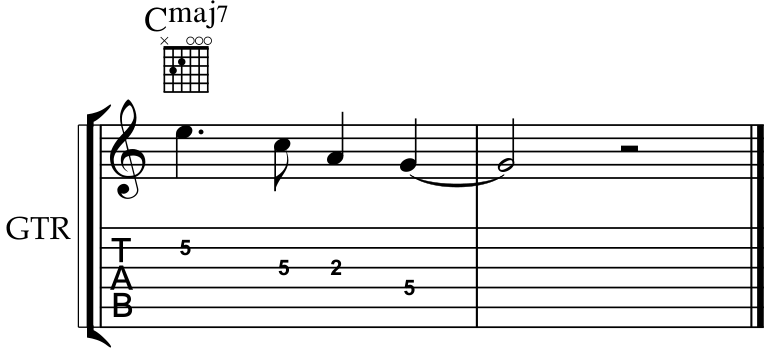
\includegraphics[width=.6\textwidth]{images/chapter2/guitarnotation.png}
            \captionsetup{width=.5\textwidth}
            \caption{An excerpt for guitar demonstrating Boulez' three main categories of notation. From top to bottom: \textit{launching}; \textit{result}; \textit{action}.}
            \label{fig:guitarnotation}
        \end{figure}

    Per Boulez' formulation, the melody given here in traditional notation is an example of ``outcome'' notation: The pitches encoded here on the top staff represent discrete sonic events with a certain predominating frequency and a certain duration: the outcome a composer hopes to achieve. The tablature beneath serves as ``action'' notation: Numbers indicate positions on the fretboard for a particular string which will ostensibly produce the desired pitches. Finally the lead-sheet symbol above (along with accompanying fretboard diagram) are examples of ``launching'' notation: prescribing creative boundaries for improvisatory action rather than sounds themselves of the same level of specificity as the other two forms. Crucially, while any of these alone might result in a sonic outcome which would satisfy a composer, they each display a radically different level of fixity. That is to say: in this example, result notation most tightly restricts the sonic outcome, followed by action notation which, taken by itself, allows for a great deal more latitude given its lack of durational values and rests (hence its frequent accompaniment by traditional notation in transcription/pedagogical texts). Launching notation, by design, only very loosely constrains the field of potential for a performer in terms of the pitch content of the sonic result. An illustration summarizing Boulez' notation typology is given in Figure~\ref{fig:Bouleztyp}.

\begin{figure}
    \centering
    \small
    \begin{forest}
                forked edges,
                for tree={draw,align=center,edge={-latex}}
                [\textsc{Notation},circle,draw
                    [\textit{Result}
                    ]
                    [\textit{Action}
                        [\textit{Launching}]
                    ]
                ]
                \end{forest}
    \caption{Boulezian typology of music notations.}
    \label{fig:Bouleztyp}
\end{figure}
    
    Much of Boulez' lecture is concerned with factors which might lead a composer to opt for one of these forms of notation over the others. He writes:

        \begin{smallquote}
            [T]o no small degree, the desire to compose comes from the contact we have with our musical heritage, our imagination naturally---necessarily---fits itself into regions defined by the lessons we have had. We think by way of them, thanks to them; and these ideas will conform to traditional kinds of notation. Yet new methods are vital when reflection intensifies our awareness of the differences between our heritage and ourselves. Using smooth time, in the realm of duration, where pulsation is no longer evident, or any point of reference to unity, and none of the multiple units of value such unity embodies, implies that we seek out either a spatial distribution that visually represents the temporal distribution we are imagining or an approximate correspondence of values for which an exact numerical correspondence is impossible.\autocite[531]{Boulez_Nattiez_2019}
        \end{smallquote}

    \noindent For Boulez, composers typically limit themselves to traditional notation because it is only from within this traditional framework that they received their training and the bulk of their musical experiences. In essence, their musical sound/process-concepts are predominantly conceived \textit{in terms of} this notation---ergo, it represents the boundaries of their musical experience. A composer who develops a new S/PC, perhaps one which relies on a notion of spatial analogy or of some form of indeterminacy, is thus best served by a notation which traces the contours of this concept.
    
    In this way, Boulez implicitly posits a sort of smooth continuum of notational fixity spanning from hyper-precise result notation intended for machine realization (e.g. a Conlon Nancarrow player piano roll); down through the less-fixed notation for Baroque and jazz performance (featuring both a high degree of latitude \textit{and} a high degree of specificity); all the way to wide-open neo-notations (``aleatoric music [...] `floating' music without pulsation'' or ``non-tempered intervals, where certain local notational features must be devised'') which may only specify one parameter, leaving the rest to interpretation.\autocite[53f6]{Boulez_Nattiez_2019} Interestingly, he makes no explicit mention of the now-common edge case that is the asemantic graphic score---that is, a certain type of (what I've been calling) ``image-first'' score---which makes no attempt to encode musical parameters at all (even while potentially gesturing at traditional glyphs, à la Cornelius Cardew's mammoth and oft-cited \textit{Treatise} 1963--7).\footnote{These asemantic works will be discussed in greater depth later in the chapter.} Neither, though, does he (directly) mention Feldmanian or Cagean graphic scores which explicitly provide keys for their interpretation. Crucially, he draws no particular distinction between these and other open notations strictly on grounds of the novelty of their encoding mechanism. 

    This wisely side-steps a problem we have not yet addressed---namely, the problem of cleanly separating what we typically think of as ``graphic'' scores from traditional or modified-traditional scores (themselves necessarily ``graphic''  insofar as they comprise written symbols as opposed to, say, strictly text). Rather, while we often categorize notations based on their appearance and the extent to which they deviate from tradition, Boulez opts to distinguish them by their \textit{function} as prescribed by either received syntax or by a composer's instructions---that is, by the way they communicate. Action, result, or launching notations might take familiar or unfamiliar forms, but in the end it is their syntax and communicative semantic content which differentiate them from one another rather than superficial properties of their physical traces.

    In the end (perhaps unsurprisingly) Boulez comes across as rather conservative when it comes to a composer's choice of notation; gently ribbing those who spring at the chance to devise radical new systems seemingly for their own sake.

    \begin{smallquote}
        With new objects [...] whose codes are presently uncertain, even non-existent, transcription becomes difficult, imprecise [...] complex to the point of uselessness[...] The problem lies in the attention required by the signs defining the object that one wants to communicate -- quantitative or qualitative. Familiar signs, newly invented signs, super-elaborate signs, deceptive signs -- a large number of solutions are available to the \textit{inventor} who might, in time, become a composer.\autocite[532]{Boulez_Nattiez_2019}
    \end{smallquote}

    \noindent Ultimately, for Boulez, new notation ought not be conceived and adopted merely as a means to mediate or alter a performer's relationship to a musical text. Rather, innovation should always be motivated by the pursuit of greater fidelity to a composer's ``object''---i.e. her sound/process-concept. I take it, though, that in many cases composers who design bespoke notations, sometimes only encoding rather simple process concepts (``play higher than $x$,'' ``play something loud!'') are taking this mediation/alteration as their brute materials---just as Boulez took pitches and durations as his---and are thus worthy of serious consideration despite their ``inefficiency.''

    This conservatism, though, does not detract from the general salience of his argument. His analytic rubric (a) focusing on notation's function over its form and (b) permitting the smooth continuum of notation's multivariate fixity is essentially the only way forward if we take as our goal a more detailed understanding of modern notation practices. These represent a significant leap forward over Eco's binaristic take on the open work and thus is one we'll carry with us as we further assay the open music practices of the twentieth and twenty-first centuries. 



    %\begin{smallquote}
    %    *****Are the two kinds of writing compatible? Does amorphousness exclude fixity by definition, or does it confront it? The two kinds of invention, gesture and state, can indeed confront one another, corroborate each other, respond, be superimposed, in any instrumental or non-instrumental domain. They can be manipulated in such ways, but one should not forget that gesture, with all this implies regarding freedom and unpredictability, remains above all the concern of the interpreter, while state is the special domain of the machine able to realise it in better, richer and more satisfying ways. [557]
    %\end{smallquote}

    %\begin{smallquote}
    %    *****In most cases one employs a notation of action, not of outcome; this is logical, since if one desires an outcome that changes every time, it would be absurd to notate one outcome and impossible to notate all outcomes. The only adequate strategy is to describe how one is to act in terms of what materials to use; hence the dichotomy, in the notation, between the elements to be used and their mode of use. [559]
    %\end{smallquote}
    
    
%    \begin{notestuff}
%       Two important takeaways that we want to bring with us: smooth continuum of fixity and defining/categorizing/taxonomizing notations based on their functions/the relations they set up between comp/perf.
%    \end{notestuff}


\subsection{Do we need an open work?}

    Confronted with Boulez' argument, the question arises: Is it actually important that we take a stab at more robustly defining the open musical work? After all, as I concluded in a prior section, all scores performed by humans are at least trivially ``open'' insofar as they all permit (demand) some degree of conscious or unconscious creative decision-making on the part of a performer before the work is able to exist---as intended---as sonic products. Each symbol, no matter how strict, merely affords a field of potential action to a player and will always contain far more than one relevant gesture; ergo, the product is not strictly regulated pre-performance; ergo it is open. Ultimately, though, this leaves us unsatisfied. Ask a pianist who has played both \textit{Structures I} and Brown's \textit{December 1952} which piece (if either) is open and which (if either) is closed. Ten times of ten they'll respond that the latter is---or at least feels---wide open. I take it that a robust notion of open works must be able to account for this experiential discrepancy; that is, it must be able to point to the most salient features of the composer/score/performer relationship which bring about this phenomenological difference.
    
    The simplest solution would be to claim that a score is open if its symbols denote sufficiently large (or ``broad'') fields of potential action. The breadth of this field is indeed one way we might think to class notational glyphs. After all, it is fairly clear (per Section 1 of this chapter) that \{$\vcenter{\hbox{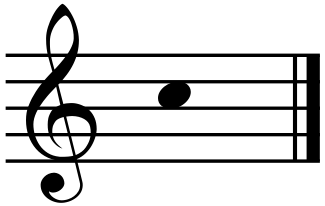
\includegraphics[width=1.2cm]{images/chapter2/c5raw.png}}}$\} affords far more potential realizations than \{$\vcenter{\hbox{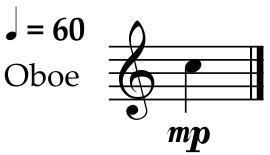
\includegraphics[width=2cm]{images/chapter2/c5oboe.png}}}$\} and thus has a broader FOP. However, it is inevitably difficult to identify, in concrete terms, magnitudes of size for these fields, given that even the ``smallest,'' most closed-off FOP permits essentially infinite realization---albeit many with vanishingly small sonic differences. Undeniably, $|FOP\{C5_{bare}\}| >> |FOP\{C5_{oboe}\}|$, but by how much? By what proportion? It remains unclear. As such, it would be untenable to categorize open works strictly according to the size of their symbols' FOP---i.e. by the sheer number of creative interpretations possible.
    
    Rather, to identify a categorical distinction characterized primarily by an \textit{experiential} difference, it would only make sense to congruently appeal to the experience of the performer. Clearly there are certain musical parameters that we as performers are accustomed to having ``held open'' in performance, despite experiencing a work as closed to creative contribution. If I, a hypothetical conservatory clarinetist, perform Stravinsky's \textit{Three Pieces for Clarinet Solo}, I experience it as a fixed work even given its inherent openness---i.e. the creative liberties afforded to an unaccompanied musician: timbre, intonation, microtiming, dynamics, etc. My experience with the piece's encoding scheme and my knowledge of the expectations which attend western concert music performance in general let me know that the larger-scale pitches, onsets, durations, and tempi are not up for negotiation and must be observed according to the score which dictates them. 
    
    When, on the other hand, I perform Louis Andriessen's \textit{Workers Union} (1975), I am suddenly presented with notation which no longer affords fixed pitches individually; or, more accurately, it affords a broad \textit{range} of pitches for each notehead present. As Boulez observed, it is often via this stripping-away of notational specificity rather than the addition of novel symbols that composers formally denote space for performer contribution. In Figure~\ref{fig:workersunion} below, Andriessen opts to encode melodic contour on a single-line staff rather than the traditional fixed-pitch five-line staff. As approximate pitch height is meant to be indicated by the relative distance from the horizontal center-line, I might begin the gesture presented at rehearsal letter \textbf{H} with a high written G$\sharp$5, A5, or A$\sharp$5, say, depending on how closely I track the spatial relationship between notehead and centerline throughout the piece.

            \begin{figure} 
            \centering
            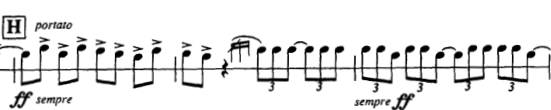
\includegraphics[width=.9\textwidth]{images/chapter2/workers_union.png}
            \captionsetup{width=.5\textwidth}
            \caption[Mm. 54--56 of Louis Andriessen's \textit{Workers Union} featuring single-line-staff notation denoting open pitches.]{Mm. 54--56 of Louis Andriessen's \textit{Workers Union} demonstrating single-line-staff open pitches.\footnotemark}
            \label{fig:workersunion}
        \end{figure}
        \footnotetext{\autocite{Andriessen_1975}}
        
    Permissible deviations in pitch have now exceeded the typical ``quantum'' unit standard notation was designed to express. Where deviations on the order of the cent are permissible (read: inevitable) from performance to performance under traditional Western classical performance conditions, Andriessen's neo-notation encodes looser constraints: repeat performances will now differ in pitch on the order of the \textit{semitone} or greater. As a clarinetist in the ensemble, the ``liberation'' of one of these typically non-negotiable musical parameters communicates to me the work's openness; striking me as an entirely new category of work. Further, while it is possible that the only noteworthy pitch deviation during Stravinsky's \textit{Three Pieces} might be my minor, unconscious shifts in intonation, at a certain level when I perform \textit{Workers Union} I must make deliberate formal commitments on the order of instrument register and specific pitch. This shifting of the domain of performance discrepancy from unconscious to conscious cognitive processes similarly renders the work ``open.'' This might explain why Berio's flute \textit{Sequenza} struck Eco as being distinct enough to include as a prime example of an open work, despite its really rather conservative affordances.\footnote{Roughly translated, its instructions read: ``The execution time and duration ratios are suggested: by the reference to a constant quantity of space which corresponds to a constant metronome beat; from the distribution of notes in relation to that constant amount of space: [empty staff showing duration of one measure at 70 M.M.]. [empty staff] is therefore equal to approximately 0.80". The [eighth-note] notes must be played free: their effective duration is suggested by the attack mode. The duration of the [multiple beamed eighth-notes] notes is intended to be extended until the next note. The value of [fermata] is ad libitum. Small notes should preferably be played as quickly as possible. The distribution ratios indicated for [fermata] and small notes are only valid as a suggestion.'' \autocite{Berio_1958}} Per Berio's instructions, onsets and durations are ``free,'' within the (fairly strict) confines designated by the given spatial proportions. This liberty is enough, though, to demand willful creative contribution from the player and ultimately to produce variances which exceed the typical discrepancy between theoretical and observed expressive attack timings (often much less than the duration of a sixteenth note); thus it strikes the player as a new sort of freedom.\autocite{Benadon_2009}

    In sum, the best way to go about arguing for a distinct category of ``open'' musical works is to appeal not to composer desires, nor the physical trace of the score, nor even to the sheer number of potential unique realizations, but instead to the phenomenal qualities of the performer's engagement with the work. If, by dint of the player's active decisionmaking, willful creativity, surprise, etc., she feels as though she's engaged with a new type of work distinct from the sometimes typewriterly experience of more traditional ``fully-notated'' music; then the work is an open one.
    
    In the end, though, there are enough edge-cases to render the initial question moot. The score for James Tenney's \textit{Having Never Written a Note for Percussion} (1971) consists entirely of one single-line staff for any percussion instrument; featuring no tempo indication, no time or key signature, and only a single rolled whole note centered on the notecard-sized page (see Fig.~\ref{fig:tenney}). 

            \begin{figure} 
            \centering
            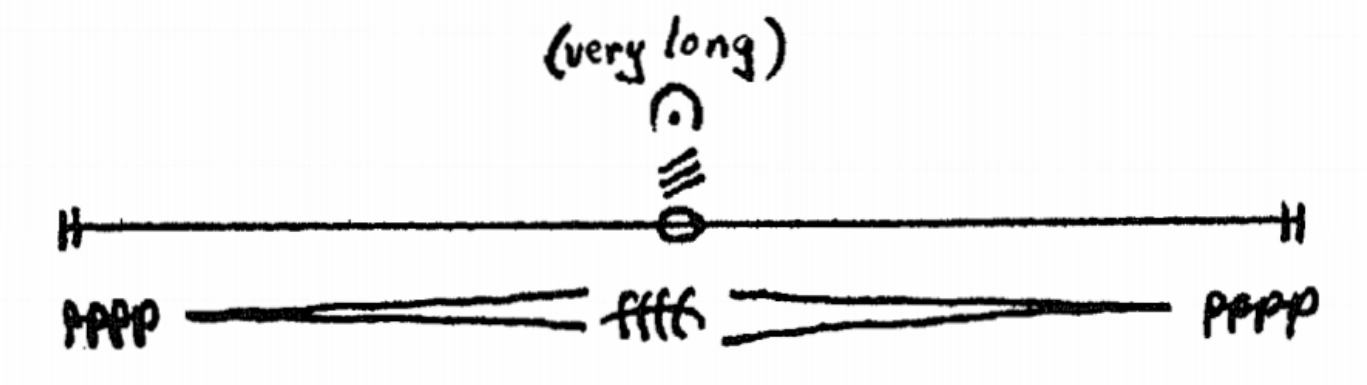
\includegraphics[width=.8\textwidth]{images/chapter2/tenney.png}
            \captionsetup{width=.5\textwidth}
            \caption[Full score of James Tenney's \textit{Having Never Written a Note for Percussion.}]{Full score of James Tenney's \textit{Having Never Written a Note for Percussion.}\footnotemark}
            \label{fig:tenney}
        \end{figure}
        \footnotetext{\autocite{Tenney_1971}}

    \noindent Performance consists of a single swell from \textbf{\textit{pppp}} to \textbf{\textit{ffff}} and back---to be played over a ``very long'' period. The total performance duration is entirely up to the performer: a small sampling of YouTube performances range from one minute to thirty. Though it is most often performed on the largest gong one can muster, any percussion instrument may be selected. Given that the whole note is of uncertain duration, the three-line tremolo indication (typically representing either an unmeasured or a thirty-second-note roll for percussion instruments) is not specific with regard to frequency of attack. Clearly, this stripped-down notation conforms well to Eco's common-sense notion of open works. To the contrary, though, the piece is \textit{experienced} as solidly fixed in place. Given that the dramatic arc of the work is so structured (i.e. with a dynamic apex right at the middle), once the performer has decided upon a particular length and a particular roll frequency, she will be able to execute the work as a singular, monadic gesture; one with as little deviation from performance to performance as would arise from a wholly-traditionally-notated version of the score. Ultimately, whether we ascribe the qualifier ``open'' to the work or not, the notation affords what it affords.

    At least as pertains to deliberately-encoded structures of notation (be they of traditional, stripped-down, or novel forms) I maintain that the notion of the ``open score'' as such is a distinction without a difference; standing in for an arbitrary point on the fixity gradient. The concept may be a useful one insofar as it serves as lexical shorthand or encourages us to think more carefully about our roles as composer or performer, but it becomes increasingly obsolete in an era characterized by ever greater intermingling of compositional and improvisatory forces---both inside the classical canon and without.


%*****When deviations cross the threshold from autonomic to deliberate...
%*****For an experiential distinction, we have to appeal to experience. Musical choices made consciously \textit{feel like} independent creative contributions---ergo their associated works will feel open. 
%*****Armed with these new concepts (FOP-signification, function classification, fixity gradient) let's revisit a few of our earlier examples from Chapter 1 to formally describe what's going on between the composer/notation/performer---maybe describing things in terms of the formal descriptors I used above.
%*****As I've already discussed, it's trivially true that all human-oriented scores are ``open'' by virtue of the impossibility of identical performances. However, based strictly on the phenomenological discrepancy between performing a hypothetically ``closed'' work like a Beethoven piano sonata and an ``open'' work like Dec '52, we desire that a refined, robust definition of an open work would account for this discrepancy.

    
% \begin{notestuff}
% %**these should be accounted for by a new model of the open work.---sometime before section 2.

% %(1) what figured-bass represents and how that differs from a lead sheet symbol

% %(2) what feldman's squares represent

% %(3) what dec 1952 represents

% %(4) Is there precedent for this view? Can we read this view into existing papers even if they don't use the same neologisms?
% *** But there's a glaring problem we haven't discussed---one that is not adequately accounted-for using strictly the terminology we've been using. There seem to be two major poles in the world of neo-notational open scores: the semantic and the asemantic. Per our earlier discussion this isn't meant to be taken as a binary but a continuum---and as such we can find many works occupying all points along this gradient. While we've looked at several works along this gradient, they all share a robust grounding in representation---even Dec. 52. 
% \end{notestuff}

\section{Steps toward a typology}

%\begin{notestuff}
%    \begin{smallquote}
%        \textbf{QUESTION TWO:} The explosion of novel notation schemes in the 1950s and 1960s presented us with a new problem: that of a certain type of ``image-first’’ score—namely ones which do not purport to encode any particular musical parameters, merely laying themselves bare for interpretation by a performer in any way s/he sees fit. To what extent ought we to consider these notation at all? They certainly represent a new sort of phenomenological experience for the performer — ought we consider them an entirely new category of music representation given they don’t ``refer’’ as such to anything?
%    \end{smallquote}
%\end{notestuff}

    Thus far we have alluded to but carefully side-stepped a big issue at the heart of contemporary notation practices. At the end of the previous chapter, I compared Feldman's \textit{Projection} series with Earle Brown's \textit{December 1952} by contrasting them as representative of ``sound-first'' and ``image-first'' styles of composition, respectively. To be clear, these labels referred not to any positive attributes of the notations themselves, but to particular modes of construction favored by the composer. Where glyphs in a ``sound-first'' arrangement would be chosen for their ability to result in a specific desired sonic outcome, ``image-first'' compositions would be constructed based on a desired visual aesthetic; allowing the sounds to arise as they may.
    
    % \begin{notestuff}
    %     I may need a sentence or two clarifying this at the end of last chapter and/or at the beginning of this one.
    % \end{notestuff}
    
    It is important that this dichotomy in notation's poiesis not be confused with one which purports to say something about notation's \textit{content}. Even using the most bog-standard traditional notation, for instance (which I take it is typically used because of the particular sounds it elicits) it is quite possible to construct scores from an ``image-first'' perspective---centering the visual results. One famous fifteenth-century example is given in Fig.~\ref{fig:heart}; albeit one whose graphicality was probably never intended to impact performance per se.
    
            \begin{figure} 
                \centering
                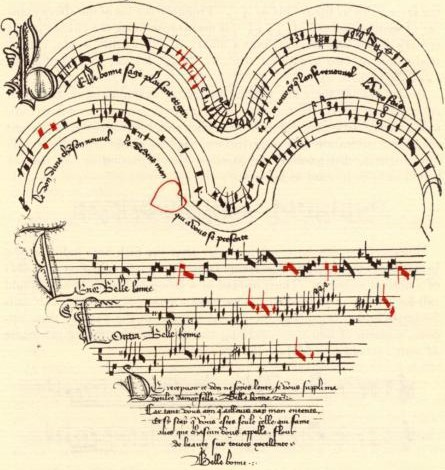
\includegraphics[width=.5\textwidth]{images/chapter2/bellebonnesage.jpg}
                \captionsetup{width=.5\textwidth}
                \caption[An early example of what might be considered ``image-first'' notation: Fifteenth-century chanson \textit{Belle, Bonne, Sage} by Baude Cordier, rendered using unconventional notation in the shape of a heart.]{An early example of ``image-first'' notation: Fifteenth-century chanson \textit{Belle, Bonne, Sage} by Baude Cordier, rendered using unconventional notation in the shape of a heart.\footnotemark}
                \label{fig:heart}
            \end{figure}
            \footnotetext{Found in the Codex Chantilly courtesy of \autocite{CHANTILLY}}
    
    \noindent On the other hand, Iannis Xenakis' electroacoustic \textit{Mycenae Alpha} (1978) (excerpted below in Figure~\ref{fig:mycenae}) is an example of ``image-first'' composition in which final sonic results are entirely contingent on the graphicality of its ``score''. Xenakis here used bespoke hardware/software to translate drawing directly into sonic contour with no performer interpretation required. What we identify as its score is really more of a complex set of computer inputs which incidentally serve as a tightly-coupled visualization.

            \begin{figure} 
                \centering
                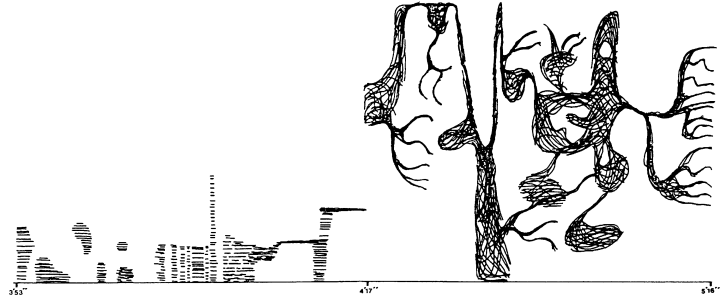
\includegraphics[width=.9\textwidth]{images/chapter2/mycenae.png}
                \captionsetup{width=.5\textwidth}
                \caption[Page 2, system 1 of Xenakis' \textit{Mycenae Alpha} (1978). Designed to be rendered precisely into sound by UPIC---bespoke visual-to-audio translation hardware/software.]{Page 2, system 1 of Xenakis' \textit{Mycenae Alpha} (1978). Designed to be rendered precisely into sound by UPIC---bespoke visual-to-audio translation hardware/software.\footnotemark}
                \label{fig:mycenae}
            \end{figure}
            \footnotetext{\autocite{Xenakis_1987}}
    
    \noindent Shifting our focus to notation's content, however, requires an entirely new formal distinction. As I hope my argument in Section 1 has demonstrated, every piece of music highlighted so far may be functionally reduced to a single type of $\text{\textit{composer}} \rightarrow \text{\textit{performer}}$ communication: a sound/process-concept is encoded for eventual transmission and execution. There exists, though, a second type of musical inscription which upends this traditional relationship by rejecting the notion that a score need necessarily encode anything at all. Neither Eco nor Boulez directly address the existence of this second type despite its consistent presence in and amongst neo-notational works since the 1940s at latest. This is not to say that their existence has gone unheeded: Many other writers have engaged with these ``asemantic'' works in one way or another, most often in the larger context of 1960s sonic indeterminacy.\footnote{For instance, Chapters 8 and 9, ``Improvisation'' and ``Indeterminacy,'' respectively in \cite{Cope_1984}; Chapter 2 ``Indeterminacy'' in \cite{Taruskin_2009d}; Chapters 2, 7, and 9 in \cite{Griffiths_2011}; etc.} Overwhelmingly, these authors fail to substantively discuss the bare function of notation and the semantic/asemantic distinction among these scores; grouping these types together under categories like ``improvisatory works,'' ``indeterminate works,'' ``aleatoric works,'' etc. Descriptors like these purport to say something about the composer's attitude toward openness, the relationship between composer and performer, and/or their desire for sonic indeterminacy---topics which of course merit discussion on their own. However, distinctions like these universally fall short of probing the actual mechanics of the works' fundamental building blocks: their inscriptions and their signs.

    Thus far my survey of relevant literature has focused on well-known and widely-published scholarship. However, by far the most thoughtful and comprehensive treatment of the taxonomy and function of new notations comes in the form of György Ligeti's little-known essay „Neue Notation: Kommunikationsmittel oder Selbstzweck?” (``New Notation---Means of Communication or an End in Itself?'') published in a special 1965 issue of the Darmstadt journal of new music.\footnote{I'd like to extend an extra special ``thank you'' to Dr. Amy Bauer for providing a provisional translation of this paper. Coincidentally, it received its first official translation into English just as I began fleshing out this chapter. It is this translation which I will cite throughout this section, though given that it has no official page numbers, I'll cite page numbers as they appear in the original German-language edition. Original paper found in \autocite{Ligeti_1965}} Given that no extant English-language scholarship discusses this fascinating article, I would like to dedicate the following section to a thorough unpacking of Ligeti's insights; extending to both this important functional dichotomy and to aspects of notation already addressed in some detail in this chapter.

    \subsection{``New Notation---Means of Communication or an End in Itself?''}

    Vis-à-vis the article's title, the main thrust of Ligeti's argument is that depending on the precise way it is deployed, a novel system of musical notation may serve either as a means of communicating desired sound-concepts from a composer to a performer, or as a standalone performance-stimulating work of art, or both. Composers make decisions about how best to represent the ultimate sonic trace of the work depending on their artistic aims. However, Ligeti, unlike many other scholars, takes great pains to differentiate systems of notation proper from what he dubs ``musical graphics''. Not to be confused with the more common usage of the term ``graphic notation,'' which we often take to mean anything distinct from traditional staff-dot-stem-beam notation, Ligeti's use of the term here parallels what I have so far called ``asemantic'' notation---i.e. deliberately un-coded.
    
    These graphics, he claims, bear the same relationship to a composition's sonic products as a drawing of a house does to the actual, three-dimensional house it represents. The drawing does not ``mean'' the house---it merely serves as a depiction; allowing one to recognize the really-existing structure in its two-dimensional contours, but not to construct the house by following detailed instructions.  This depiction (of the sound or of the house) does not rise to the level of a sign in that it does not stand in a logically consistent network alongside other graphic depictions. 

    We might once again take Cardew's \textit{Treatise} as an example (minimally excerpted below in Figure~\ref{fig:Treatise1}):

            \begin{figure} 
                \centering
                \fbox{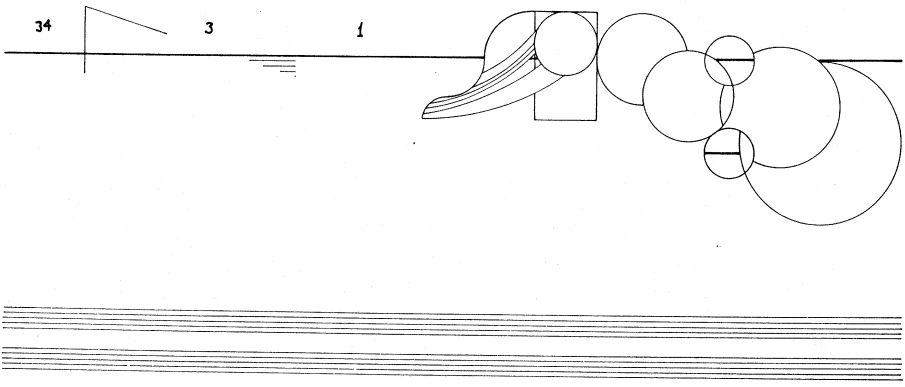
\includegraphics[width=.9\textwidth]{images/chapter2/cardewtreatisepg1.png}}
                \captionsetup{width=.5\textwidth}
                \caption[First page of Cornelius Cardew's asemantic magnum opus, \textit{Treatise}(1967).]{First page of Cornelius Cardew's asemantic magnum opus, \textit{Treatise} (1967).\footnotemark}
                \label{fig:Treatise1}
            \end{figure}
            \footnotetext{\autocite{Cardew_1967}}

    \noindent Famously, despite an enigmatic gesturing toward traditional notation in the form of the clefless grand staff at the bottom of the page, the ``symbols'' used in the piece's construction (numbers, line segments, overlapping circles, etc.) bear no composer-mapped semantic content. Construction of meaning is left entirely as an exercise to the interpreter. Insofar as one particular inscription can not be said to stand in any particular relationship to any other (save spatially), Ligeti takes these sorts of scores as comprising not notation, but something wholly separate.

    For Ligeti, notation proper\footnote{To avoid confusion, I'll use ``notation proper'' to refer to Ligeti's understanding of the term; distinguishing it from common usage.} necessarily forms an internally coherent system unto itself whose inner relationships bear some resemblance to the system of relationships present in the final sonic object---a system wherein notational glyphs (serving as signs) are laden with semantic content and which ``[correspond] to a system of auditory processes'' rather than standing in for sound directly.\autocite[pg. 171 in Ernst et al., 1965.]{Ligeti_forthcoming} He emphasizes that a means of scoring may only be dubbed ``notation'' so long as some means of inter-translatability exists between it and another coherent system of signs. Just as we could freely translate between (to use his example) FORTRAN and programmers' punch cards, so may we translate between traditional notation and, say, the ``piano roll'' notation used in digital audio workstations. Attempting to translate an asemantic graphic score in the same way would inevitably result in failure, Ligeti claims; thus it can't be considered notation at all but a wholly distinct type of composition. Over the course of the following section, Ligeti goes on to establish a tentative typology; one which seeks to encompass every form of what we might generally call ``music inscriptions,'' focusing primarily on breaking down the many varieties of notation proper and using several contemporary pieces as apropos case-studies. For posterity and toward the defense of my own views, I will describe this typology here.

    At the top hierarchical level sit the aforementioned ``notation'' and ``graphics,'' cleanly separated by their contents: coherent relations with other signs on one side and pictorial marks on the other. Notation is divided into  two primary categories: what he calls ``result notation'' (\textit{Resultatnotation}) and ``realization notation'' (\textit{Realisationsnotation}).\footnote{Notably similar to but distinct from Boulez' own categories.} Result notation is by far the most deterministic. So dubbed because it is ultimately the sonic result which is depicted on the page, result notation is used when uncertainty between the scored ``map'' and the final sonic ``territory'' ought to be kept to a minimum. Most traditional notation, for instance, falls into this category. As it is typically deployed, a transcription can result in a near one-to-one mapping between image and sound. Result notation is also used in scored electronic music where frequencies, durations, linear/nonlinear movement, etc. have been mapped with exacting precision graphically. Here, Ligeti cites an excerpt from Friedrich Cerha's ``Mouvement II'' from \textit{Mouvements I-III} which precisely represents moment-to-moment changes in pitch using glissando curves---accurately visually mapping the frequency content present for each instrument.

    % \begin{notestuff}
    %    If I decide to keep Boulez, I need a paragraph or so contrasting Boulez' language to Ligeti's---and noting his lack of attribution.
    % \end{notestuff}

    Realization notation\footnote{...which, confusingly, Boulez would later refer to as ``action notation''...} serves instead as guidelines for actions which, if successfully performed will ``realize'' the desired sonic output. Realization notations ``may be totally clear, partly clear, or unclear,'' depending on the practical needs of the composer and the desired level of fidelity between the score and product. As realization notations become increasingly complex and precise, Ligeti claims, they begin to approach result notation in the tightness of their coupling to resultant sound.\autocite[pg. 178 in Ernst et al., 1965.]{Ligeti_forthcoming}

    This realization notation is itself further divided into two categories---``action notation'' (\textit{Aktionsnotation}) and ``recipe-'' or ``formula notation'' (\textit{Rezeptnotation}). Recipe notation is perhaps easier to grasp, occurring when a composer lays out perfectly clear step-by-step instructions describing what the performer must do to achieve a desired sound. This notation is often formulated as textual instructions (e.g. ``softly strike a twelve-inch diameter tom-tom at the two-o'clock position one inch from the rim three times quickly'') but also includes tablature notations which (as mentioned earlier in the chapter) describe the precise positioning of the hands and fingers necessary to sound as the composer intends. Recipe notation, unlike result notation, bears no direct parallels to the resultant sound. Instead, it is deployed in scenarios where (a) multiple paths exist which would result in a desired sound (and the composer seeks to isolate a single path for the performer) or (b) where notating the performer's step-by-step movement is ultimately more economical than encoding the resulting sound; notating the twist of a knob, for example, rather than the complex sonic output of a synthesizer.

    Action notation, on the other hand, is on balance the least deterministic of the group. Like formula notation, it too exists to demonstrate a space of action to a performer which will result in a given sound or range of sounds when physically emulated. However, rather than providing a clear step-by-step recipe, it illustrates a visual analogy that the performer must interpret. Ligeti here cites the non-deterministic notation for the organ (which many others would incorrectly class as ``graphic'') found in Mauricio Kagel's 1972 \textit{Improvisation ajoutée} (Fig.~\ref{fig:kagel1}). 

        \begin{figure} 
        \centering
        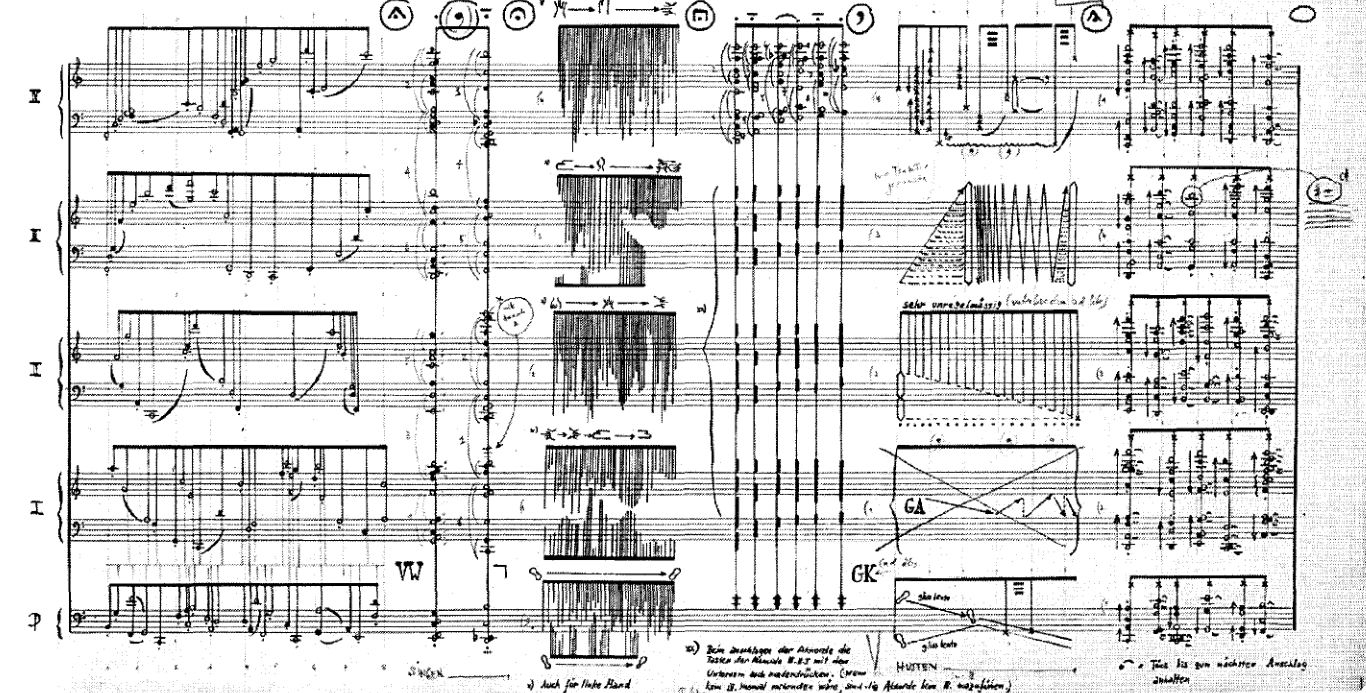
\includegraphics[width=1\textwidth]{images/chapter2/kagel1.png}
        \captionsetup{width=.5\textwidth}
        \caption[Excerpt of Mauricio Kagel's \textit{Improvisation ajoutée} (1972) courtesy of Ligeti's original paper.]{Excerpt of Mauricio Kagel's \textit{Improvisation ajoutée} (1972) courtesy of Ligeti's original paper.\footnotemark}
        \label{fig:kagel1}
    \end{figure}
        \footnotetext{\autocite[181]{Ligeti_1965}}

    Here we find glyphs seemingly based on traditional stems and beams, but impossibly tightly-packed into such a small space that a performer could not be reasonably expected to execute their attacks with a traditional level of ``faithfulness'' to the sign. Thus the performer must directly analogize their own physical gestures with the visual representation shown on the staff---the result being necessarily less precise than the sonic output of a result notation. Below in Figure~\ref{fig:Ligtyp} I've provided a tree diagram summarizing the above description of Ligeti's hierarchy of notation types (contrast with Figure~\ref{fig:Bouleztyp} above).

\begin{figure}
    \centering
    \small
    \begin{forest}
                forked edges,
                for tree={parent anchor=south, child anchor=north,draw,align=center,edge={-latex}}
                [{\textsc{Inscription}},circle,draw
                 [Notation\\(proper)
                    [{\textit{Result}}, tier=word
                    ]
                    [{\textit{Realization}}
                        [{\textit{Action}},tier=word
                        ]
                        [{\textit{Recipe}},tier=word
                        ]
                    ]
                ]
                 [{Graphic},tier=word
                 ]
                ]
                \end{forest}
    \caption{Ligetian typology of music notations.}
    \label{fig:Ligtyp}
\end{figure}

 Crucially, his rendering includes space for signs and systems which do not conveniently fall into one of the above categories---without which, any attempt to theorize notation would be woefully incomplete. Ligeti describes ``intermediate forms'' which demonstrate attributes of both symbolic notation and musical graphics, of which Brown's \textit{December 1952} is his prime example.\footnote{It seems here that Ligeti, like Griffiths, was under the mistaken impression that \textit{December 1952} lacked any preambulatory text or instructions. His argument is based on this assumption and thus treats the work like a particularly well-structured ``graphic'' rather than a notation as such. We'll bracket this oversight for now, as it doesn't particularly impact the thrust of his argument.} Ligeti interprets Brown's work as both a graphical work unto itself as well as a formally delimiting agent; setting distinct (though imprecise) boundaries for performer interpretation via its visual arrangement. Ligeti claims:

\begin{smallquote}
    If [\textit{December 1952}] is realized musically, there are numerous possibilities---and yet the interpretation is not totally free, because the visual configuration sets quite definite limits. In this regard, this musical graphic also possesses some (rudimentary) elements of a sign system.\autocite[pg. 177 in Ernst et al., 1965.]{Ligeti_forthcoming}
\end{smallquote}

\noindent Ultimately, these hybrid forms not only serve as intriguing case-studies by which we might contemplate the nature of composer/performer agency, but also lend further credence to Ligeti's typology insofar as they demand separate analysis of the function of their constituent symbolic/graphic components. ``[T]he fact that the sign component can be separated from the graphic aspect within mixed forms,'' he claims, ``is itself a demonstration that we are dealing with two fundamentally different categories.''\autocite[pg. 177 in Ernst et al., 1965.]{Ligeti_forthcoming}

In the end, Ligeti argues that the composer's decision to deploy either a system of (neo-) notation or a pseudosystem of musical graphics rests on a question of desired ``adequacy, clarity, and economy'' in musical representation. His thesis here relies on a vivid analogy which takes the purely graphic score to be the \textit{map} of a particular (sonic) territory and the notated score to be the walking of a \textit{single path} through that territory. The musical graphic is both richer and more ``wasteful'' in that, like the map, it contains innumerable details pertaining to countless ``hikes'' that cannot be experienced in a single journey. In the act of performative interpretation, one necessarily discards every unrealized detail in favor of the chosen path. The ``single walk,'' on the other hand, has its own inner richness in that it is able to reveal features invisible on the map---foregoing potential variety of experience for finer-grained detail and ``paripeteias'' otherwise inaccessible to such a zoomed-out view. The decision to enlist either the map or the path thus rests on the extent to which a composer seeks reproducibility and fine-grainedness or the richness of unlimited, irreproducible detail.\autocite[pg. 178 in Ernst et al., 1965.]{Ligeti_forthcoming}

Because, Ligeti  claims, scored instrumental and vocal music always retains some ``margin of vagueness'' when contrasted with fixed electronic music, and because this vagueness is always already intimately tied up with the notational markings used to represent a flexible, imprecise music, systems of notation will tend to reflect this flexibility and imprecision. Thus, as contemporary composition varies wildly in its degree of determinism from piece to piece (and even within pieces!), pure one-size-fits-all systems of notation tend to be eschewed in favor of meta-systems which hybridize characteristics from pure graphics, result notation, action notation, and recipe notation depending on the particulars of the composition in question. The notation used to encode Kagel's \textit{Improvisation ajoutée}, per Ligeti's example, succeeds not because it attempts to be unified and all-encompassing, but precisely because of the extent to which it hybridizes notations spanning Ligeti's typology: result notation in the form of determinate pitches, action notation for the organists hands and feet, and formula notation for entabulating the organ's stops.\autocite[pg. 180 in Ernst et al., 1965.]{Ligeti_forthcoming}

% \begin{notestuff}
%     Boulez' complaint from earlier about the prevalence of bespoke, non-standardized solutions could be seen to be in response to this mashing together of different notation schemes without a sort of meta-theory guiding their use.
% \end{notestuff}

\subsection{Why are Ligeti's typology and analysis valuable to us today?}

Ligeti's appraisal of the structure and use of these distinct forms of notation and graphics, perhaps owing to his practical, composerly experience with many of these forms, is strikingly refined in contrast to other historical and contemporary takes on the matter. As such, I take it that further elucidation of this typology might be of some use in the study of notation and of ``open'' composition today. Ligeti is one of only a few scholars to draw a firm distinction between methods of music inscription on grounds of their semantic content or lack thereof---that is, on whether they denote concrete musical materials or merely connote potential spaces of action. Where many authors ambiguate these two antipodean categories under the label ``graphic notation,'' ``indeterminate notation,'' etc., for Ligeti, the fundamental property of an inscription is not its novelty, but its contents.

Under Ligeti's formulation, the fixity of a notational glyph or set of glyphs does not necessarily correlate one-to-one with the strength of its semantic content. A functional, logically coherent sign system may have highly-fixed sounds or gestures as its points of reference, as in the precisely-engraved result notation of a piece of electronic music. On the other hand, a similarly coherent, denotative notation may point to highly \textit{indeterminate} sounds or gestures---for instance, the dense, headless grace-note figures from \textit{Improvisation ajoutée} or Feldman's pitch-range notation. These figures are notational rather than graphic in the sense that while the performer's creative act of reading will vary significantly from performance to performance, the composer had a key role in determining the bounds of that semantic content (and therefore in predictably influencing the sonic products resulting from the figures' realization).

As such, Ligeti separates notation's relative fixity or openness from its ability to meaningfully communicate. One might imagine a less nuanced view, whereby a glyph's communicative potential is strictly proportional to the quantity of its fixed content. A mode of inscription totally lacking sonic specificity would thus be unable to effectively communicate anything at all. Given, though, that many such sonically indeterminate works (including wholly asemantic works) enjoy repeat performances and some form of persistent identity, we should prefer to say that they retain  communicative potential, despite their irreducibility to one particular sound world. We might represent these opposing univariate and bivariate views using ``denotative'' to indicate the presence of composer-provided semantic content and ``connotative'' to indicate its absence (Fig.~\ref{fig:typologies}).

\begin{figure}
    \centering
            \begin{tabular}{ |c|c| }
             \hline
             \multicolumn{2}{|c|}{\textbf{Traditional univariate typology}} \\
             \hline
             fixed and denotative & open and connotative  \\ 
             \hline
            \end{tabular}

                \vspace{10pt}

            \begin{tabular}{ |c|c| }
             \hline
             \multicolumn{2}{|c|}{\textbf{Ligetian bivariate typology}} \\
             \hline
             fixed denotative & \textcolor{gray}{fixed connotative\footnotemark}  \\ 
             \hline
             open denotative & open connotative  \\     
             \hline
            \end{tabular}
    \caption{Univariate vs. bivariate notation typologies.}
        \label{fig:typologies}
    \end{figure}
            \footnotetext{``Fixed connotative" notation is a category merely implied by the existence of its antitheses. This is as-yet untheorized as it would require a notation which is somehow ``defined" by its interpreter but which is nonetheless semantically stable across performance scenarios. The lack of a well-defined ``fixed connotative" notation forces me to refer to fixity and content as only ``quasi-independent" rather than truly independent properties.}

    \noindent While under the old view, notation's content is directly proportional to its fixity, only concretely denoting insofar as its sonic products are predictable, under Ligeti's new bivariate view, notation may strongly denote regardless of the indeterminacy of its products.

    To elaborate on this distinction: Here, ``fixed denotative'' notation describes that which has been rendered systematic ahead-of-time by the composer or by received practice. The final sonic trace of the work is more-or-less predictable/replicable because the notation hews closely to the final sonic product. Note that this is to say nothing of how closely it resembles traditional notation in its printed form; traditional notation does indeed fit into this category---but so does, say, the widely-adopted ``cipher'' tablature commonly used to notate Indonesian gamelan compositions (Fig.~\ref{fig:gamelannot}).

    \begin{figure}
        \centering
        \fbox{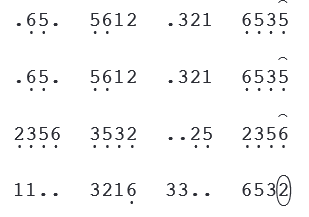
\includegraphics[width=.4\textwidth]{images/chapter2/gamelancipher}}
        \captionsetup{width=.5\textwidth}
        \caption[\textit{Nut angka} contemporary style of gamelan notation demonstrating an excerpt of \textit{Gending Titipati sléndro pathet nem}.]{\textit{Nut angka} contemporary style of gamelan notation demonstrating an excerpt of \textit{Gending Titipati sléndro pathet nem}.\footnotemark}
        \label{fig:gamelannot}
    \end{figure}
        \footnotetext{\autocite{Ishida_2008}}

    \noindent The ``open connotative'' type, on the other hand, describes what Ligeti calls musical graphics---asemantic drawings which have no ahead-of-time systematicity. These figures only have meaning insofar as it is given by the interpreter, either pre-performance or in-the-moment (hence connotative). The quasi-symbols depicted on the page merely ``suggest'' musical moves; the final sonic products are entirely downstream of the performer's decision to (or refusal to) map glyphs to gestures themselves.
    
    %The formal distinction between ``open connotative'' and ``open denotative'' notation represents a significant point of refinement for Ligeti's view over those of his peers.
    
    Finally, the ``open denotative'' category refers to the structures of notation that have thus far been the primary topic of this study---specifically those in which symbols explicitly encode desired fields of potential action, but deliberately leave space for willful creative interpretation on the part of the performer. In other words, they bear semantic content (hence denotative) but maintain an indeterminate sonic trace. Per Section 1, the particular quality and quantity of semantic ``data'' they bear is merely a function of the specificity with which it shapes the field of potential action afforded to a performer. 

    Where Figure~\ref{fig:Ligtyp} demonstrated Ligeti's typology as expressly relayed in his article, Figure~\ref{fig:Amendtyp} below refines this typology by making explicit the implied categories of semantic-fixed and semantic-open notations (again, distinct from asemantic, connotative notations). Note that, per earlier discussion, these categories do not represent a hard binary but rather two poles delineating a smooth gradient.

    \begin{figure}
    \centering
    \small
    \singlespacing
    \begin{forest}
                forked edges,
                for tree={parent anchor=south, child anchor=north,draw,align=center,edge={-latex}}
                [\textsc{Notation},circle,draw
                 [{\textbf{Denotative}}
                    [{Semantic\\fixed}, name=A
                        [{\textit{F. Res.}},tier=word]
                        [{\textit{F. Real.}}
                            [{\textit{F. Act.}},tier=word]
                            [{\textit{F. Rec.}},tier=word]
                        ]
                    ]
                    [{Semantic\\open}, name=B
                        [{\textit{O. Res.}},tier=word]
                            [{\textit{O. Real.}}
                                [{\textit{O. Act.}},tier=word]
                                [{\textit{O. Rec.}},tier=word]
                            ]
                    ]
                ]
                 [{\textbf{Connotative}}
                    [{Asemantic\\open},tier=word]
                 ]
                ]
                \draw[<->,dotted] (A)  to[out=east,in=west] (B);
                \end{forest}
    \captionsetup{width=.5\textwidth}
    \caption{Refined Ligetian typology of music notations. Dotted arrow indicates presence of ``fixity gradient'' between the semantically fixed and open genera.}
    \label{fig:Amendtyp}
\end{figure}
    
    %For Ligeti, notations proper are divisible into his distinct subcategories (result, action, recipe) only because of their ability to properly encode and transmit composerly intent. The strictly connotative ``graphics'' on the other hand are essentially brute fact---differentiable only by the qualities of their inscription.

    Among Ligeti's many observations, the relatively intuitive division of musical inscription into two fundamental categories---the semantic/denotative and the asemantic/connotative---represents a significant point of refinement for typologies of notation in general. I take it that this (in conjunction with his subcategories of notation proper) permits a more nuanced understanding of mid-century sonically-indeterminate notations and their descendants than is typical of the field. Let us take, for example, two works from the same time period which make extensive use of neo-notation: John Cage's \textit{Concert for Piano and Orchestra} (1957--8) (see Fig.~\ref{fig:cagepiano1}) and No. 1 from Sylvano Bussotti's \textit{Five Piano Pieces for David Tudor} (see Fig.~\ref{fig:bussottipiano1}). 

    \begin{figure}
        \centering
        \fbox{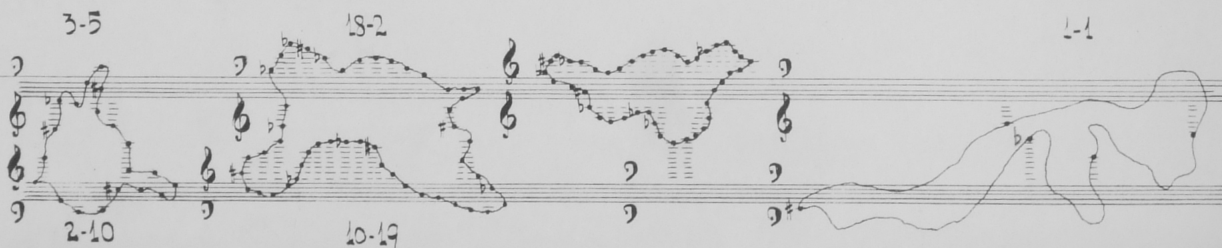
\includegraphics[width=.99\textwidth]{images/chapter2/cagepianomoduleL.png}}
        
            \vspace{10pt}
            
        \fbox{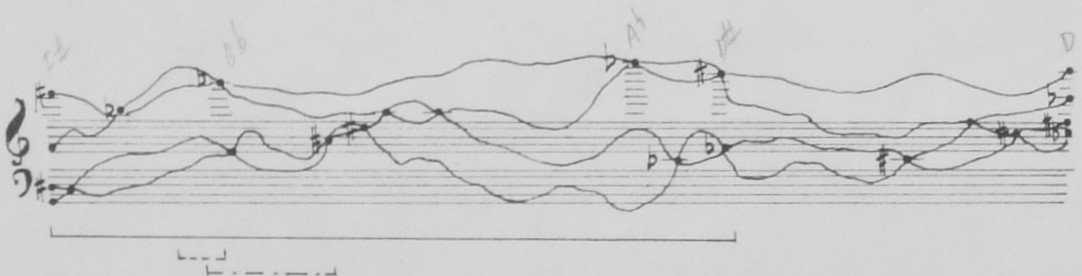
\includegraphics[width=.99\textwidth]{images/chapter2/cagepianomoduleM.png}}
        \captionsetup{width=.5\textwidth}
        \caption[Modules ``L'' and ``M'' from the piano solo of Cage's \textit{Concert for Piano and Orchestra} (1957--8).]{Modules ``L'' and ``M'' from Cage's \textit{Concert for Piano and Orchestra} (1957--8).\footnotemark}
        \label{fig:cagepiano1}
    \end{figure}
        \footnotetext{\autocite{Cage_1960}}

    \begin{figure}
        \centering
        \fbox{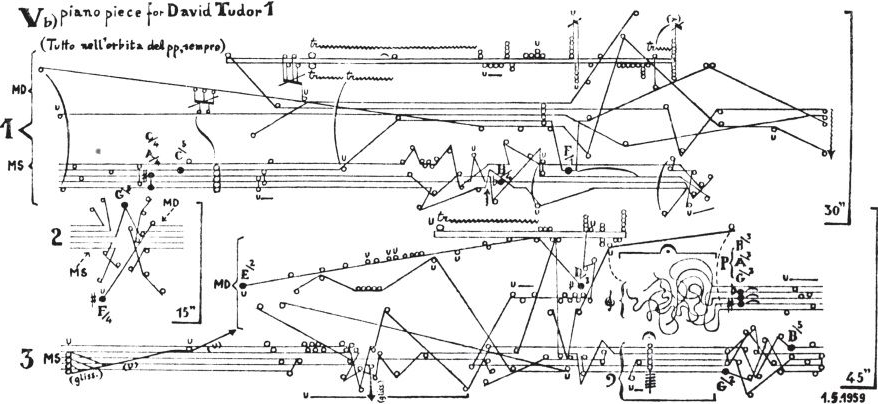
\includegraphics[width=.99\textwidth]{images/chapter2/BussottiPiece1.png}}
        \captionsetup{width=.5\textwidth}
        \caption[Full score of No. 1 from Sylvano Bussotti's \textit{Five Piano Pieces for David Tudor} (1959).]{Full score of No. 1 from Sylvano Bussotti's \textit{Five Piano Pieces for David Tudor} (1959).\footnotemark}
        \label{fig:bussottipiano1}
    \end{figure}
        \footnotetext{\autocite{Bussotti_1959}}

        At first blush, there are many commonalities between these two excerpts. Both are pieces for unaccompanied piano which ground the performer in their sense of musical literacy by using familiar glyphs: staves, clefs, points which might represent attacks, linear or curved connectors. Both are clearly sonically indeterminate; requiring a significant degree of creative interpretation for their realization. The critical distinction between the two is that while Cage's piano solo came packaged with detailed instructions defining the boundaries of successful interpretation (excerpted below for context)...

    \begin{smallquote}
        \noindent \textsc{[...] the whole is to be taken as a body of material presentable at any point between minimum (nothing played) and maximum (everything played), both horizontally and vertically [...]}
    \end{smallquote}
        \vspace{-20pt}
    \begin{smallquote}
        \noindent \lettrine[lines=2, findent=3pt, nindent=0pt]{B}{:} \textsc{[...] the single staff is provided with 2 clef signs. where these differ, ambiguity obtains in the proportion indicated by the 2 numbers above the aggregate, the first of these applying to the clef sign above the staff.} [...]
    \end{smallquote}
        \vspace{-20pt}
    \begin{smallquote}
        \noindent \lettrine[lines=2, findent=3pt, nindent=0pt]{L}{:} \textsc{play from left to right with hands indicated. clef ambiguity as in B. perimeters were composing means and do not here affect time, as they do in a.}        
    \end{smallquote}
        \vspace{-20pt}
    \begin{smallquote}
        \noindent \lettrine[lines=2, findent=3pt, nindent=0pt]{M}{:} \textsc{begin at left, end at right, changing direction at intersections if desired. may be expressed as one voice, a `counterpoint,' or as 3 or 4 voices. pedals only in areas indicated, not obligatory.}\autocite[pg. B]{Cage_1960}
    \end{smallquote}




    \noindent ...Bussotti's instructions for his piece for Tudor begin and end with the Italian inscription at the top of the page: ``All in the orbit of \textbf{\textit{pp}}, always.'' 
    
    While Cage's work inarguably compels a performer to interpret its symbols creatively, it does so by restricting (with lesser or greater degrees of rigor) the performer's field of potential using the symbols' semantic content which Cage himself encoded. To use Ligeti's terminology: the floating noteheads are examples of result notation in that they ought to result in the sounding of particular pitches.  The ``aggregates'' of which they are members, though, are forms of action notation in that they provide a visual/spatial analogy for onset/duration to which the performer must hew. The text block preceding the piece is a sort of recipe notation insofar as it expressly denotes conditions for successful interpretation. Bussotti's work, on the other hand, predominantly comprises Ligetian ``musical graphics'' in that (beyond the initial inscription) the piece relies \textit{entirely} on performer interpretation. Its familiar appearance and sprinkling of recognizable glyphs belie the fact that Bussotti intended the work in its entirety to serve as ``launching'' notation (to use Boulez' term); essentially in contravention of all received notions of musical literacy. Bracketing the \textit{pianissimo} indication, any constraint on the potential action of the performer is up to the performer herself.

    Many authors expressly or implicitly make the case that Cage and Bussotti's works from this period represent two adjacent ideological camps with regard to performer liberation---both employing a similar compositional language with Bussotti merely taking the marginally more ``radical'' tack in his permissiveness. What Ligeti illuminates, however, is that owing to their semantic structures, these two inscriptions represent two entirely distinct classes of ``writing,'' with appropriately distinct structures of agency. Both are ``graphic'' in the colloquial sense of the term in that they depart from standard music encoding methods, but the approaches are miles apart when it comes to their actual function. Not coincidentally, Stockhausen selected works from the two series represented here when he conducted his 1959 Darmstadt lecture series entitled ``\textit{Musik und Grafik}'' (diligently analyzed by David Gutkin in \textit{Perspectives of New Music} (2012)). Though I lack the space to fully detail Stockhausen's (or Gutkin's) observations on what were then brand-new structures of notation, it's clear that both he and Gutkin take Bussotti's piano pieces to comprise a sort of implicit action notation; though one which ``only effects actions in a very indeterminate matter.''\autocite[276]{Gutkin} While they note that Bussotti's inscriptions represent a basically new compositional method, they fail to articulate that an entirely new relationship is set up between composer (here ``inscriber'') and performer---one in which essentially all \textit{restrictive} capactity belongs to the interpreter while the inscriber serves only to ``provoke'' or ``incite'' action by connotation.\footnote{Gutkin's paper is, by and large, an incisive and much-needed look at a fascinating and under-studied sector of music theory. He reads far deeper into the function and significance of strictly connotative notation than I am prepared to do here---I merely take issue with this particular characterization of Bussotti's work.} 
    
    To illustrate, I've included another interaction model (Fig.~\ref{fig:graphicdiagram}) to reflect the function of musical graphics (to contrast with that of notation proper). Noteworthy differences include: (1) The initial sound-concept becomes superfluous, the score is now merely an instance of \textit{ekphrasis}---a drawing ``about sound'' but one ultimately informed by a graphic- (rather than a sound-) concept. (2) The score merely \textit{connotes} a field of potential to the performer who (3) encounters the notation via \textit{gazing} (per Gutkin's term), producing sound which bears no necessary semantic connection to the graphic itself.

        \begin{figure} 
            \centering
            \fbox{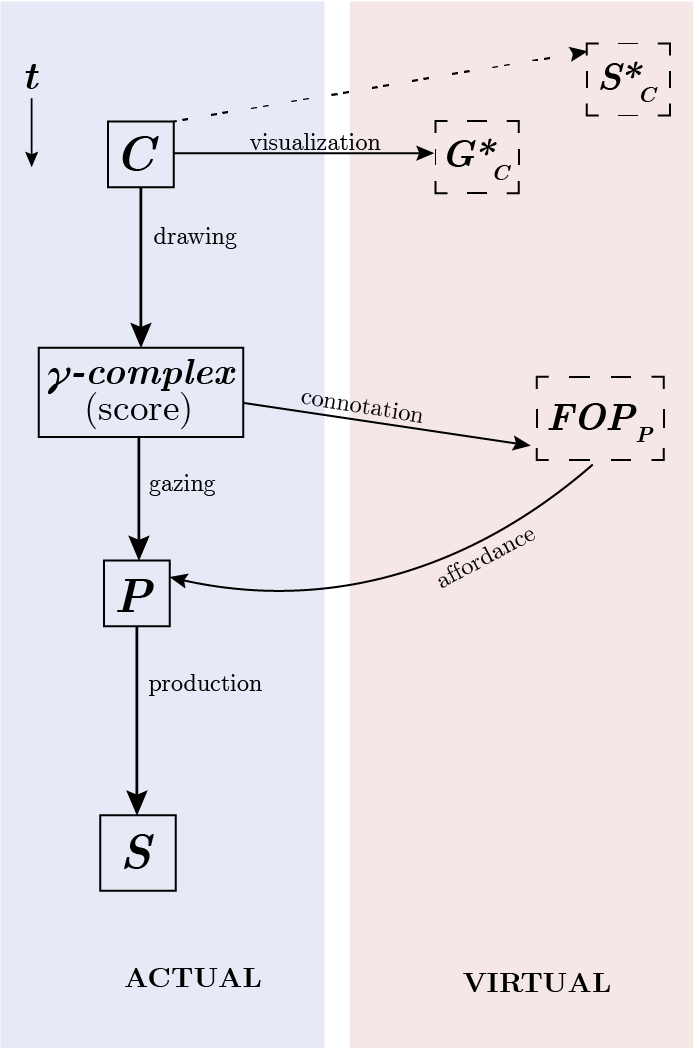
\includegraphics[width=.5\textwidth]{images/chapter2/graphic_signification_diagram.png}}
            \captionsetup{width=.5\textwidth}
            \caption{``Graphic'' interaction model---to contrast with that of notation proper.}
            \label{fig:graphicdiagram}
        \end{figure}

    As far as my interests are concerned, though, the most pertinent strength of Ligeti's typology lies in its ability to meaningfully describe ``hybrid'' works/notations---i.e. compositions which integrate, often at quite a granular level, instances of denotative and connotative notations. If we accept his analysis that semantic and asemantic inscriptions, (``sign system'' and ``illustration'') are two fundamentally distinct categories which nevertheless may ``grow into one another,'' I take it that there are two fundamental mechanisms by which this hybridization may occur.\autocite[pg. 177 in Ernst et al., 1965]{Ligeti_forthcoming}
 
    First: Over the course of a score, section of a score, or even a single gesture, a composer may employ conventionally-coded symbols (of either traditional or neo-notation) \textit{alongside} asemantic inscriptions to be freely interpreted. We might dub this style ``concatenative'' hybridity. Figure~\ref{fig:revis} illustrates one such example which I engraved for Eric Revis in 2021. Painted ``background'' portions were provided with no accompanying code and were meant to provide improvisatory grounding for the traditionally- (or mostly-traditionally-) notated floating fragments.

        \begin{figure} 
            \centering
            \fbox{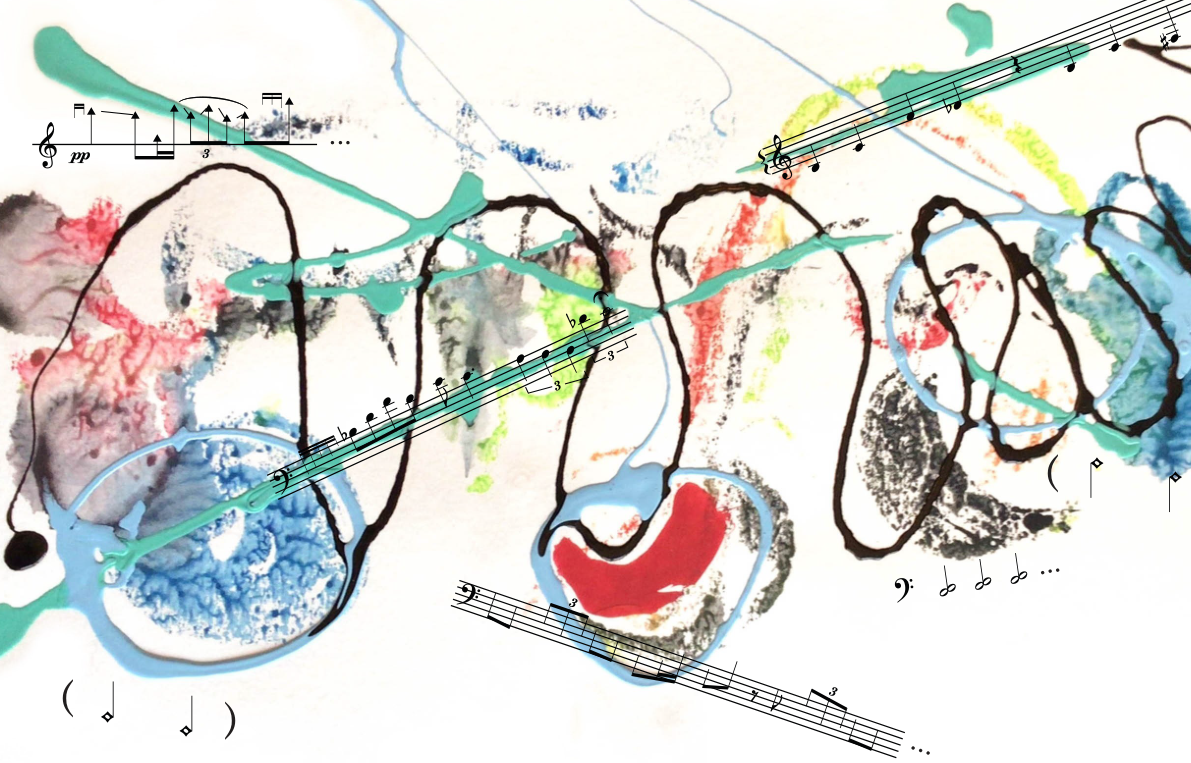
\includegraphics[width=.9\textwidth]{images/chapter2/slipknots2.png}}
            \captionsetup{width=.5\textwidth}
            \caption[Score created \textit{ex post facto} for Eric Revis' ``Slipknots Through the Looking Glass \#2'' demonstrating ``concatenative'' hybridity. Traditional and modified-traditional notations are used side-by-side with non-coding graphics.]{Score created \textit{ex post facto} for Eric Revis' ``Slipknots Through the Looking Glass \#2'' demonstrating ``concatenative'' hybridity. Traditional and modified-traditional notations are used side-by-side with non-coding graphics.\footnotemark}
            \label{fig:revis}
        \end{figure}
            \footnotetext{Original performance by Eric Revis. Painting by Ayanna Bassiouni. Transcription/engraving by Isaac Otto. Recording from \autocite{Revis_2020}.}

    Second: A single conventionally-coded symbol (either traditional or neo-notation) \textit{itself} might demonstrate noteworthy ``graphicality''---an ability to connote despite its separate, robust encoding---what we might dub ``simultaneous'' hybridity.\footnote{We might consider a third type: a semantically-coded symbol accompanied by or involving inscriptions which are strictly \textit{incidental}; neither coded to constrain a field of potential action nor designed to incite performer-mapping. It's unclear whether we ought to even consider this ``graphic excess'' notation of any sort, or whether it's best thought of as mere decoration. We might consider \textit{Belle, Bonne, Sage} shown above in Figure~\ref{fig:heart} to be an example of this third mechanism---perhaps ``decorative'' hybridity.} I take Cathy Berberian's \textit{Stripsody} (1966) (shown in Fig.~\ref{fig:stripsody1} below) to be a canonical example of this second form. Berberian provides explicit instructions for the interpretation of glyphs insofar as they conform to traditional ${time}\times{pitch}$ mapping on the $x$- and $y$-axes and standard notions of proportional duration/onset. However, each glyph (word) also demonstrates an ``excess'' of graphicality beyond simple decoration; presumably meant to influence the execution of that symbol in ways that remain un-coded. 

        \begin{figure}
            \centering
            \fbox{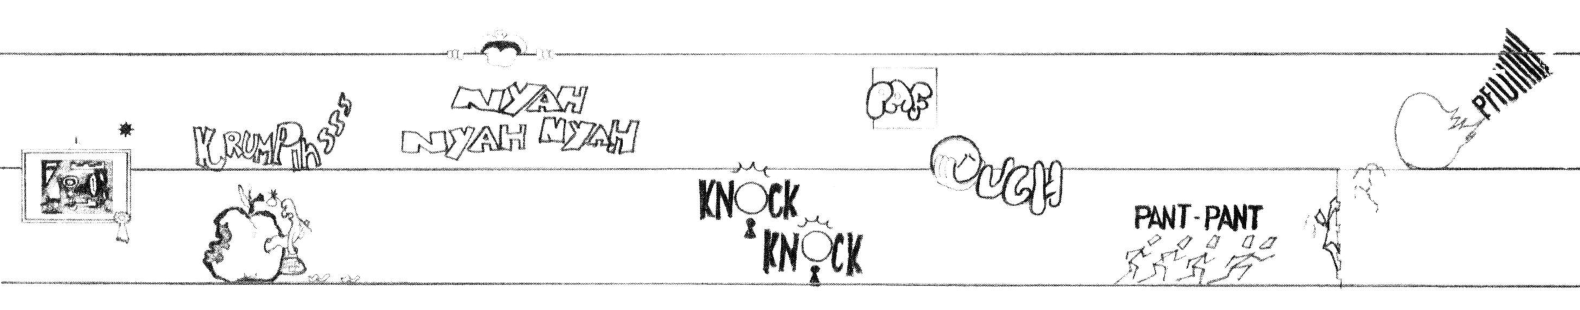
\includegraphics[width=.99\textwidth]{images/chapter2/stripsody1.png}}
            \captionsetup{width=.5\textwidth}
            \caption[System three on page four of Cathy Berberian's \textit{Stripsody} (1966) demonstrating ``simultaneous'' hybridity. Coded symbols themselves demonstrate connotative potential---i.e. ``graphicality.'']{System three on page four of Cathy Berberian's \textit{Stripsody} (1966) demonstrating ``simultaneous'' hybridity. Coded symbols themselves demonstrate connotative potential---i.e. ``graphicality.''\footnotemark}
            \label{fig:stripsody1}
        \end{figure}
             \footnotetext{\autocite{Berberian_1966}}

    Naturally, some questions remain: At what point may one claim that a notational symbol crosses over into meaningful graphicality---i.e. when does a symbol become sufficiently affective as to be able to impact performance via connotation? Precisely in which ways does this graphic excess serve to impact performance? On which factors is this graphic mediation contingent? At this point, answers to these questions would be essentially speculative, though it now seems possible to ask them empirically; in such a way that their answers might fall in the empirical domain of performance psychology and music cognition. Ultimately, I would argue that the mere ability to meaningfully raise these questions represents a new degree of subtlety in the discourse surrounding notation which would not be possible without Ligeti's analysis.


% \begin{notestuff}
%     Begin wrap-up here. Just make the claim that with the tools laid out by Ligeti and some subtle re-rendering we are much better equipped to assess what's going on in these multi-layered scores; how they work; what they afford
% \end{notestuff}
    
% \begin{notestuff}
%     *****The recognition of the existence and value of HYBRID notations I think is where a lot of the meat is. When composers (like Cage in his Concert) use deliberately evocative notations, they're in fact hybridizing two entirely different mechanisms: the restrictive and the inciting.  
% \end{notestuff}

%         \begin{notestuff}
%         \begin{center}
%         GUTKIN ARGUMENT
%         \end{center}
        
%         *****Cage and Bussotti are often discussed as two points along a continuum -- Cage still reliant on explicit instructions for the interpretation of his figures and Bussotti even more radical; allowing for any mapping desired by the performer. However these are b est understood as entirely different paradigms, which Ligeti understood! Even Stockhausen via Gutkin seems to get this wrong. These are two fundamentally different kinds of thing. These things can be HYBRIDIZED but I wouldn't call it a continuum. The mapping comes from two different places! Notation function ``flow'' chart is different! 
        
%         The vestigial notation-like glyphs on the page might provoke similar responses from performers but the fact remains that it's all performer-oriented. This is what so many seem to miss. Tudor recognized this in his transcription/performance of the Bussotti ``The piece \textit{is} the lines and the surfaces on the paper.'' (Gutkin 272)  
        
%         Signification =/= Stimulation (Gutkin 273) 
        
%         *****He's right that there's always an element of ``gazing'' in ``reading'' (pg. 277) but the reverse isn't necessarily true. No meaningful semantic communication occurs in the Bussotti and it's our responsibility to be able to differentiate these things so that we might see hybrid works as complexes of the two actions---reading and gazing.
%         \end{notestuff}

% \begin{notestuff}
%     \begin{center}
%         COPE ARGUMENT
%     \end{center}
% \begin{smallquote}
%     *****Improvisation differs from indeterminacy, as its meaning in music refers to the aspect of performer interaction, an activity more often than not controllable in rough shape by the composer, and even predictable within limits.\autocite[244]{Cope_1984}
% \end{smallquote}

%     *****Improvisation is more a notational than a philosophical challenge to tradition.\autocite[242]{Cope_1984}

%     Cope selects a bunch of open, denotative notation and works to demonstrate ``improvisation,'' but also includes William Duckworth's largely asemantic \textit{Walden Variations}. Then in his section on ``performer indeterminacy'' in the next chapter, he does precisely the same thing---including several pieces with open denotative symbols (traditional or neonotation) and then asemantic neonotation in the form of John Mizelle, Robert Moran, etc. He claims that these are notational distinctions but doesn't make an effort to differentiate the notations that characterize these two ``different'' music-making paradigms.

%     Per Ligeti's formulation, the distinction between ``improvisation'' and ``performer indeterminacy'' is strictly academic. Notated works are reducible to the function of their symbols.

%     *****Cope notes that certain pieces (bussotti) feature ``nonsymbolic abstract representation'' (282) for which ``interpretation or noninterpretation is fully within the performer's realm'' but doesn't meaningfully distinguish between these notations and those which robustly encode musical parameters. He refers to Cage's style of notation as ``somewhat graphic'' (277) without explaining what that might mean. Both of these works he categorizes as ``performer indeterminacy'' along with traditionally notated but cellular works like Stockhausen's Klavierstuck XI.
%     \end{notestuff}


    
% \begin{notestuff}
%     \begin{itemize}
%         \item Contrast with Cope's mixed-up improvisation/indeterminacy dichotomy?? At least in order to illustrate the value of Ligeti's (and my) much more performance-grounded reading of notation-mediation...
%         \item An amended notation typology    
%     \end{itemize}
% \end{notestuff}

\section{Conclusion}

To synopsize the main takeaways from the discussion presented in this chapter:

(1) It often behooves our analysis of the form and function of music notations to consider them not pictorial representations of past or potential future sounds, per se, but rather as generic coded instruction sets which denote particular mediated fields of potential musical action in performance. In order to serve as a music notation, these instruction sets must internally cohere according to a received syntax, arrived at either via the accretion of interpretive norms acquired over the course of a performer's musical education and experience, or given explicitly via the score itself.

(2) If we seek fuller understanding of the complex, multiform notations which have become more commonplace since the 1950s (and which show no sign of disappearing anytime soon!), it is important to have at our disposal a well-defined notation typology. This should address not only the graphic trace of the inscriptions used to mediate performance, but should also take into account their various mechanisms of action.

(3) Developing these definitions requires that we disabuse ourselves of certain antiquated notions surrounding the performance of scored music: namely, the notion that we might meaningfully distinguish ``open'' works from traditional ``fixed'' works. More robust definitions of extant notations should bear out that openness is a fundamental property of \textit{all} human-performed music, including music encoded using traditional methods. The more meaningful question, then, is ``In what way does this notation serve to mediate this music's openness?''

(4) As far back as the late 1950s, composers and scholars contemplated the properties, significance, and merit of new notations designed to enact sonically-indeterminate (i.e. ``open'') music. I've argued here that György Ligeti's (only recently-translated) 1965 essay stands as a valuable untapped resource demonstrating an uncommon degree of insight into these problems surrounding notation. To wit, Ligeti describes a function-oriented notation typology separating semantic notation proper from asemantic graphics. Further, notation as such is classed according to the means by which it restricts performers fields of potential action---into result, action, and recipe notations. I assert that a modified Ligetian typology provides us with a valuable new set of tools with which to assess the way notation (and other musical inscription) mediates the often complex relationship between composers, musical texts, and performers.

In the following chapter, I will use these tools to examine two late twentieth-century work-complexes by artists who have shown particular sensitivity in their use of neo-notations. These examples exist between and beyond commonly-understood notational binaries; demonstrating either deliberate ``traversal'' of the gradient between fixed and open denotative notations or poignant hybridity between the denotative and the connotative (or indeed both). 

% \begin{notestuff}
%     (There are, of course, a whole bunch of things I omitted for space---I want to at least pay lip service to them to make it clear that (some of) these omissions were intentional, but maybe I should save that for a kind of ``epilogue/future research'' bit of text after the final chapter?)
% \end{notestuff}

    % \subsection{The relative prominence of ``image-first'' or ``connotative'' scores}
    
    % \subsection{Fixity as independent variable}


% \begin{notestuff}
%     \textbf{\textit{This should go in a section of ch. 2 actually.}}
%     \textbf{Why are the ``image-first'' scores comparatively popular?} 
%     To be forthright: the following work primarily concerns not pieces in the ``image-first'' Brownian model, but rather those in the other, less-discussed ``sound-first'' mode. Of the many books and essays which pay lip service to this time of notational tumult in experimental art-musics, only very few do the work of actually pulling apart these radically disparate methodologies. ``Image-first'' open scores often have a strong aesthetic appeal by dint of the fact that their construction centered on imagery first; often directly inspired, as Brown's work was, by abstract visual art which took point, line, plane, and color as their first principles rather than pitch, duration, and timbre. As such, they are inevitably eye-catching---lending themselves well to reproduction and consumption by audiences who might be curious as to the nature of cutting-edge experimental music, but who lack the means to interpret more ``sophisticated'' scores which rely on \textit{encoded} musical gesture. Further, where ``graphic'' scores \textit{are} reproduced, their accompanying instructions are often fragmentary or totally absent (as was the case in Griffith's otherwise thorough chapter on the New York School). Thus works which may have been, say ``richly-encoded'' at the time of their conception are often mistaken for bare images; purely visual stimuli to be opaquely ``interpreted'' by a performer. 
    
%     I take it, too, that many of these ``visual-first'' scores lend themselves better to certain performance practices. An ensemble (be they dabblers in improvisation or dyed-in-the-wool improvisers) may find a score more approachable if it demands a high degree of performer input via creative decision-making rather than  if it demands a rigorous decoding process. As such, these ``sound-first'' open scores are often given short shrift in the relevant literature and scant sources even take the time to differentiate them from their more ``interpretive'' cousins. 
% \end{notestuff}


%%%%%%%%%%%%%%%
% END COPY %%%%
%%%%%%%%%%%%%%%
